\chapter{Guide d'Utilisation de l'Application}

\section{Introduction}
Ce chapitre présente le guide d'installation et d'utilisation de l'application \textbf{\appname}. Il
s'adresse d'abord au technicien qui installe le serveur et les postes de travail, puis aux utilisateurs :
administrateur, directeur, secrétaire, enseignant, étudiant, planificateur et développeur. Chaque
fonctionnalité est décrite selon le même canevas : objectif, chemin d'accès, prérequis éventuels, étapes
numérotées, règles et contrôles appliqués par l'application, résultat attendu et capture d'écran.

Trois conventions sont utilisées dans tout le chapitre. Le chemin d'accès suit la barre latérale, de
groupe à page, par exemple \emph{Menu > Élèves > Répertoire des élèves}. Les libellés entre guillemets
désignent des boutons ou des champs réellement présents à l'écran ; ils sont affichés dans la langue de
l'interface et sont donnés ici en français. Enfin, les règles de refus décrivent ce que le serveur
vérifie : une action grisée dans l'interface reste refusée si elle est appelée autrement, car le
processus principal relit toujours le rôle et le périmètre de l'appelant.

\section{Guide d'Installation}
\subsection{Besoins de Déploiement}
\begin{itemize}
    \item \textbf{Un serveur local} : un poste Windows qui héberge PostgreSQL 15 ou 16, avec une adresse
          \ac{IPv4} fixe (l'installation de référence utilise \texttt{192.214.23.15}), le port
          \texttt{5432} ouvert sur le réseau local et un partage \ac{SMB} pour les fichiers
          (\texttt{\textbackslash\textbackslash 192.214.23.15\textbackslash eNoteFiles}) ;
    \item \textbf{Une connexion réseau} : un réseau local filaire ou Wi-Fi, sans accès Internet
          nécessaire ; le débit doit suffire aux écritures concurrentes de quelques dizaines de postes ;
    \item \textbf{Un ou plusieurs postes clients} : Windows x64, ou Linux x64 avec les paquets
          AppImage, Debian ou l'archive portable. Aucun navigateur n'est requis : l'application est un
          programme de bureau autonome ;
    \item \textbf{Un compte applicatif} : le rôle PostgreSQL \texttt{enote\_app}, propriétaire de la base
          \texttt{eNote}, distinct du superutilisateur \texttt{postgres} réservé à l'administration du
          serveur ;
    \item \textbf{Un espace de stockage partagé} : les photos des personnes, les documents de cours et
          les captures d'anomalie sont écrits sur le partage, jamais dans la base ni sur le disque du
          poste.
\end{itemize}
Le tableau \ref{tab:ports} récapitule les flux réseau à autoriser.

\begin{table}[H]
\centering
\caption{Flux réseau du déploiement}
\label{tab:ports}
\begin{tabularx}{\textwidth}{l l X}
\toprule
\textbf{Service} & \textbf{Port} & \textbf{Usage} \\
\midrule
PostgreSQL & TCP 5432 & Toutes les lectures et écritures de l'application \\
Partage SMB & TCP 445 & Photos, documents, captures et installateurs \\
HTTP / HTTPS & 80 / 443 & Non utilisés par \appname ; laissés à une autre application du serveur \\
\bottomrule
\end{tabularx}
\end{table}

\textbf{N.B. :} le déploiement de référence a été vérifié sur un réseau local isolé, avec des postes
Windows x64 et Linux x64, une base PostgreSQL 15/16 et un partage SMB. Les étapes serveur de ce guide
sont rédigées pour Windows ; un poste Linux consomme le même serveur par \ac{TCP} et par un montage
CIFS.

\subsection{Étapes d'Installation}
\subsubsection{Côté Serveur}
\begin{enumerate}
    \item \textbf{Attribuer l'adresse fixe} : dans les propriétés de la carte réseau, fixer l'adresse
          \texttt{192.214.23.15}, le masque \texttt{255.255.255.0} et la passerelle du réseau. Vérifier
          ensuite que l'adresse répond depuis un poste client avant de poursuivre.
    \item \textbf{Installer PostgreSQL hors ligne} : transférer l'installateur officiel par support
          amovible, choisir un mot de passe pour le superutilisateur \texttt{postgres}, conserver le
          port \texttt{5432} et sélectionner les outils en ligne de commande (\texttt{psql},
          \texttt{pg\_dump}, \texttt{pg\_restore}).
    \item \textbf{Autoriser les connexions du réseau local} : dans \texttt{postgresql.conf}, fixer
          \texttt{listen\_addresses = '*'}. Dans \texttt{pg\_hba.conf}, ajouter une règle
          \texttt{host eNote enote\_app}, réseau \texttt{192.214.23.0/24}, méthode
          \texttt{scram-sha-256}. Les fichiers de référence sont fournis dans
          \texttt{deploy/server}.
    \item \textbf{Ouvrir le pare-feu} : exécuter en administrateur
          \path{deploy/server/setup-firewall.ps1}, qui ouvre le port \ac{TCP} 5432 et active le partage
          de fichiers Windows. Le script ne touche ni au port 80, ni au port 443, ni à MySQL : une
          application web déjà installée sur le serveur continue de fonctionner.
    \item \textbf{Redémarrer le service} : \texttt{Restart-Service postgresql*} pour appliquer la
          configuration. Le journal du service doit mentionner l'écoute sur toutes les interfaces.
    \item \textbf{Créer le rôle et la base} : exécuter la commande \texttt{psql -U postgres -f} avec le
          script \path{deploy/server/01-init-enote.sql}, après avoir remplacé le mot de passe de
          \texttt{enote\_app}. Le script crée le rôle, la base \texttt{eNote} en \ac{UTF-8}, accorde les
          privilèges sur le schéma et pose les privilèges par défaut pour les tables futures.
    \item \textbf{Importation de la base de données} : sur le serveur de référence, restaurer une
          sauvegarde vérifiée avec \path{deploy/server/restore-db.ps1}. Sur une installation neuve,
          charger le dump complet du schéma, puis exécuter
          \path{deploy/server/02-bootstrap-admin.sql}.
    \item \textbf{Créer le compte initial} : le script d'amorçage crée le compte \texttt{admin} avec le
          mot de passe \texttt{admin}. Ce mot de passe doit être changé dès la première connexion,
          depuis \emph{Paramètres > Votre compte > Mot de passe}.
    \item \textbf{Préparer le stockage partagé} : exécuter, dans une console PowerShell élevée,
          \path{deploy/server/setup-share.ps1}. Le script crée \texttt{C:\textbackslash eNoteFiles} et
          ses sous-dossiers (\texttt{person\_photos}, \texttt{documents}, \texttt{library},
          \texttt{screenshots}), le compte local \texttt{enote\_files} — mot de passe sans expiration,
          car un poste resté éteint un trimestre doit encore ouvrir le partage — puis le partage
          \texttt{eNoteFiles} avec le droit \emph{Modifier} pour ce seul compte. Le partage n'est pas
          ouvert à \texttt{Everyone} : c'est ce compte, et lui seul, que les postes emploient. Les
          droits NTFS doivent également autoriser l'écriture : un partage permissif sur un dossier en
          lecture seule provoque un échec de téléversement. Le script affiche enfin les trois lignes à
          recopier dans le préréglage des postes. L'application crée elle-même les
          sous-dossiers de classement : \texttt{documents\textbackslash MAJOR\_CODE\textbackslash
          CHAPTER\_CODE\textbackslash LESSON\_CODE} pour les documents de cours et \texttt{library\textbackslash
          TYPE\textbackslash CATEGORY\_CODE} pour la bibliothèque.
    \item \textbf{Configurer la sauvegarde} : planifier l'exécution nocturne de
          \path{deploy/server/backup-db.ps1} (par exemple à 23 h 00) avec une rétention de trente jours,
          et vérifier régulièrement qu'un fichier de sauvegarde est bien produit. Une sauvegarde jamais
          testée n'est pas une sauvegarde.
\end{enumerate}

\subsubsection{Côté Client Windows}
\begin{enumerate}
    \item \textbf{Construire les paquets} : sur une machine de construction connectée, exécuter
          \texttt{npm ci} puis \texttt{npm run build}, puis \texttt{npx electron-builder --win --x64}.
          Deux artefacts sont produits : un installateur NSIS et une version portable.
    \item \textbf{Installer le client} : exécuter l'installateur, ou lancer directement la version
          portable. L'installateur crée les raccourcis du bureau et du menu Démarrer ; la version
          portable ne demande aucun droit administrateur.
    \item \textbf{Déposer le préréglage de connexion} (méthode recommandée) : exécuter
          \path{deploy/client/install-preset.ps1} avec l'hôte, le port, la base, l'utilisateur, le mot
          de passe et la racine de stockage. Le fichier \texttt{deployment.json} est écrit dans le
          dossier \texttt{\%ProgramData\%\textbackslash eNote} et s'applique à tous les comptes de la
          machine. Il porte aussi le compte du partage (\texttt{smbUser}, \texttt{smbPassword}) : le
          client ouvre la session \ac{SMB} lui-même, sans qu'aucun lecteur réseau ne soit mappé. Les
          variables \texttt{ENOTE\_SMB\_USER} et \texttt{ENOTE\_SMB\_PASSWORD} remplacent ces deux
          champs sur un poste donné, sans toucher au fichier partagé.
    \item \textbf{Ou configurer la connexion manuellement} : au premier lancement, le bouton
          \emph{Server settings} de l'écran de connexion permet de saisir l'hôte, le port, la base,
          l'utilisateur et le mot de passe, puis de tester la connexion. Le voyant passe au vert et
          affiche \emph{Connected to 192.214.23.15}.
    \item \textbf{Se connecter} : utiliser le compte fourni par l'administrateur. Un compte suspendu
          après cinq mots de passe erronés est refusé avant même la comparaison du mot de passe.
    \item \textbf{Vérifier} : ouvrir le répertoire des élèves, téléverser une photo, générer un rapport
          \ac{PDF} et vérifier que l'arabe s'affiche correctement.
\end{enumerate}

\subsubsection{Côté Client Linux}
\begin{enumerate}
    \item \textbf{Installer le paquet} : copier l'AppImage et la rendre exécutable, installer le paquet
          Debian, ou extraire l'archive portable dans un dossier local. Le partage SMB ne doit pas
          servir d'emplacement d'exécution.
    \item \textbf{Monter le partage} : installer \texttt{cifs-utils}, créer un point de montage
          (\texttt{/mnt/enote}) et monter le partage avec les options \texttt{uid} et \texttt{gid} de
          l'utilisateur du bureau, sans lesquelles les téléversements échouent.
    \item \textbf{Renseigner un chemin POSIX} : la racine de stockage doit être \texttt{/mnt/enote} et
          non un chemin UNC, car le client construit les chemins avec les séparateurs du système.
    \item \textbf{Déposer le préréglage} : pour une installation Debian, un fichier machine
          \texttt{/opt/eNote/deployment.json} s'applique à tous les comptes ; pour une AppImage, le
          fichier personnel est \texttt{\textasciitilde/.config/eNote/deployment.json}.
    \item \textbf{Se connecter et vérifier} : les contrôles sont les mêmes que sous Windows ; seule la
          commande de vérification du port change.
\end{enumerate}

\subsection{Vérification de l'Installation}
Le tableau \ref{tab:verification} reprend les contrôles à effectuer sur le premier poste. Ils doivent
tous réussir avant de déployer les autres postes.

\begin{table}[H]
\centering
\caption{Contrôles de vérification après installation}
\label{tab:verification}
\begin{tabularx}{\textwidth}{c X X}
\toprule
\textbf{\#} & \textbf{Contrôle} & \textbf{Résultat attendu} \\
\midrule
1 & \texttt{ping 192.214.23.15} & le serveur répond \\
2 & \texttt{Test-NetConnection 192.214.23.15 -Port 5432} & \texttt{TcpTestSucceeded : True} \\
3 & \texttt{Test-Path "}\texttt{\textbackslash\textbackslash 192.214.23.15\textbackslash eNoteFiles"} & \texttt{True} \\
4 & Lancer le client & voyant vert : \emph{Connected to 192.214.23.15} \\
5 & Se connecter avec le compte initial & la page \emph{Overview} s'ouvre \\
6 & Ouvrir un dossier et une leçon & les textes latin et arabe s'affichent nettement \\
7 & Générer un rapport individuel & le \ac{PDF} s'ouvre avec la bonne mise en page \\
8 & Téléverser une photo & l'image apparaît et le fichier est présent sur le partage \\
9 & Ouvrir une photo sur un poste jamais mappé & l'image s'affiche : le client a ouvert la session du partage \\
\bottomrule
\end{tabularx}
\end{table}

\subsection{Mise à Jour des Clients}
\textbf{Objectif :} remplacer une version ancienne sur les postes sans intervention manuelle, depuis le
réseau local.\par
\textbf{Accès :} construction hors ligne, partage \texttt{installers}, puis \emph{Paramètres >
Administration > Version client requise}.\par
\begin{enumerate}
    \item Incrémenter la version du projet et reconstruire l'installateur sur une machine de
          construction.
    \item Copier l'installateur dans le dossier \texttt{installers} du partage, sans le renommer.
    \item Écrire le manifeste \texttt{latest.json} avec le numéro de version, le nom du fichier et son
          empreinte SHA-256. Le client refuse tout fichier dont l'empreinte ne correspond pas.
    \item Publier le même numéro de version dans \emph{Version client requise}, puis enregistrer.
    \item Au démarrage et toutes les trente minutes, un client plus ancien affiche un écran de mise à
          jour, copie l'installateur depuis le partage, le vérifie et propose un redémarrage.
\end{enumerate}
\textbf{Règles et contrôles :} une base injoignable ou un partage inaccessible ne déclenche jamais
l'écran de mise à jour, afin qu'une panne ne soit pas confondue avec une obligation de mise à jour. La
version publiée est stockée dans la base partagée ; la vider désactive le contrôle. Les postes Linux se
mettent à jour en remplaçant l'AppImage, en installant le nouveau paquet Debian ou en extrayant la
nouvelle archive.\par
\textbf{Résultat attendu :} tous les postes exécutent la version attendue, et un fichier altéré ou
incomplet est rejeté avant installation.

\subsection{Dépannage Courant}
\begin{table}[H]
\centering
\caption{Symptômes et remèdes les plus fréquents}
\label{tab:depannage}
\begin{tabularx}{\textwidth}{p{6.2cm} X}
\toprule
\textbf{Symptôme} & \textbf{Cause et remède} \\
\midrule
Voyant rouge, \emph{Not connected} & Le service PostgreSQL est arrêté, écoute seulement en local, ou le
pare-feu bloque 5432. Vérifier le service, \texttt{listen\_addresses} et la règle de pare-feu. \\
\texttt{FATAL: no pg\_hba.conf entry} & L'adresse du poste n'est pas couverte par \texttt{pg\_hba.conf}.
Ajouter le sous-réseau puis recharger la configuration. \\
\texttt{Password authentication failed} & Mot de passe différent de celui du préréglage, ou méthode
d'authentification incompatible. Réinitialiser le rôle et corriger le fichier de déploiement. \\
Un téléversement échoue & Droits insuffisants sur le partage ou montage CIFS en lecture seule. Vérifier
le partage, les droits NTFS et les options \texttt{uid}/\texttt{gid}. \\
Photos et documents introuvables, base joignable & Le poste n'a pas de session avec le partage, ou le
compte du préréglage est refusé. La ligne \emph{Resource storage} du démarrage nomme la cause :
identifiants refusés, session concurrente d'un autre compte, partage absent, serveur injoignable ou
droits insuffisants. \\
Le client exige une mise à jour & La version publiée est supérieure à celle du poste. Publier
l'installateur et le manifeste, ou vider le champ de version pour lever le contrôle. \\
\bottomrule
\end{tabularx}
\end{table}

\section{Fonctionnalités Communes}
\subsection{Tutoriels de l'application : Tutoriel Étape par Étape}
\textbf{Objectif :} expliquer une page au moment où l'utilisateur l'ouvre, avec les étapes qui
correspondent à son rôle.\par
\textbf{Accès :} bouton \emph{Guide} dans l'en-tête de chaque page.\par
\begin{enumerate}
    \item Ouvrir la page concernée, puis cliquer sur \emph{Guide}.
    \item Lire le résumé, qui tient en une phrase, puis la liste numérotée des étapes.
    \item Fermer le dialogue et exécuter les étapes ; le guide reste accessible sans quitter la page.
    \item Rouvrir le guide après un changement de rôle : les étapes propres aux autres rôles ne sont
          plus affichées.
\end{enumerate}
\textbf{Règles et contrôles :} le guide est filtré par les rôles du compte connecté. Une page sans guide
n'affiche pas le bouton ; une page dont toutes les étapes concernent un autre rôle n'affiche rien. Le
contenu est embarqué dans l'application et ne dépend d'aucun service.\par
\textbf{Résultat attendu :} l'utilisateur sait par où commencer sans documentation externe.

\begin{figure}[H]
    \centering
    \IfFileExists{images/commun_guide.png}{\includegraphics[width=0.85\textwidth]{images/commun_guide.png}}{\fbox{[[Capture : images/commun\_guide.png]]}}
    \caption{Guide étape par étape d'une page}
    \label{fig:commun_guide}
\end{figure}

\subsection{Tutoriels de l'application : Tutoriel Vidéo}
\textbf{Objectif :} montrer les gestes d'un rôle en vidéo, sans connexion Internet.\par
\textbf{Accès :} Menu > Support > Tutoriels vidéo, ou depuis la page d'aide.\par
\begin{enumerate}
    \item Choisir le rôle dans la liste : administrateur, directeur, secrétaire, planificateur,
          enseignant, étudiant ou développeur.
    \item Lancer une séquence ; la vidéo est lue dans l'application.
    \item Utiliser les commandes du lecteur pour revenir en arrière ou mettre en pause.
\end{enumerate}
\textbf{Règles et contrôles :} les fichiers vidéo sont livrés avec l'application et non téléchargés.
Un rôle sans enregistrement conserve sa place et affiche un emplacement réservé, ce qui évite qu'une
section disparaisse entre deux versions. Les séquences sont classées par nom de fichier, ce qui permet
de les numéroter.\par
\textbf{Résultat attendu :} chaque rôle dispose d'un parcours vidéo consultable hors ligne.

\begin{figure}[H]
    \centering
    \IfFileExists{images/commun_videos.png}{\includegraphics[width=0.85\textwidth]{images/commun_videos.png}}{\fbox{[[Capture : images/commun\_videos.png]]}}
    \caption{Tutoriels vidéo classés par rôle}
    \label{fig:commun_videos}
\end{figure}

\subsection{Mode Clair, Mode Sombre et Palettes}
\textbf{Objectif :} adapter l'interface à la luminosité du poste et à la préférence de l'utilisateur.
\par
\textbf{Accès :} menu du compte > \emph{Apparence}, ou \emph{Paramètres > Apparence}.\par
\begin{enumerate}
    \item Choisir l'apparence : clair, sombre, noir absolu ou suivi du système.
    \item Choisir la palette d'accent : émeraude, rouge, or ou bleu.
    \item Régler l'échelle de l'interface (pourcentage) si les caractères sont trop petits.
    \item Choisir le mode de mouvement : \emph{Performance} pour les animations, \emph{Économie
          d'énergie} pour les supprimer.
\end{enumerate}
\textbf{Règles et contrôles :} le choix est conservé sur l'appareil, pas sur le compte : deux postes
peuvent différer. L'apparence pilote aussi les surfaces natives (listes déroulantes, calendriers) et
l'icône de la fenêtre ; la palette d'accent teinte l'icône de la barre des tâches et la notification.
Le noir absolu reste un choix explicite : le mode \emph{système} ne bascule jamais en noir pur. Le mode
économie d'énergie et la préférence système de réduction des animations suppriment la transition
circulaire de changement de thème.\par
\textbf{Résultat attendu :} l'interface est lisible dans l'éclairage du poste, et le choix survit au
redémarrage.

\begin{figure}[H]
    \centering
    \IfFileExists{images/commun_theme.png}{\includegraphics[width=0.85\textwidth]{images/commun_theme.png}}{\fbox{[[Capture : images/commun\_theme.png]]}}
    \caption{Sélecteur d'apparence et de palette}
    \label{fig:commun_theme}
\end{figure}

\subsection{Support Multilingue}
\textbf{Objectif :} travailler en anglais, en arabe ou en français, y compris pour les libellés venus de
la base.\par
\textbf{Accès :} bouton de langue dans l'en-tête, l'écran public et l'écran de connexion.\par
\begin{enumerate}
    \item Choisir la langue ; l'interface se recharge immédiatement.
    \item En arabe, vérifier que la barre latérale passe à droite et que les tableaux s'inversent.
    \item Ouvrir une fiche de référence : le libellé s'affiche dans la langue active, avec la variante
          de l'autre langue entre parenthèses lorsque les deux existent.
    \item Saisir un nom de personne dans les deux écritures (latine et arabe) lorsque le formulaire le
          propose.
\end{enumerate}
\textbf{Règles et contrôles :} l'anglais sert de langue de repli : une entrée absente du dictionnaire
s'affiche en anglais plutôt que de laisser une clé technique. Le changement de langue remonte l'arbre
des composants, ce qui recharge les données de chaque page avec les libellés de la langue choisie. Le
choix est local à l'appareil et ne modifie ni le compte ni les données. Les noms de personnes ne sont
pas « traduits » : la forme latine et la forme arabe coexistent.\par
\textbf{Résultat attendu :} l'application est utilisable dans les trois langues, sans redémarrage.

\begin{figure}[H]
    \centering
    \IfFileExists{images/commun_langue.png}{\includegraphics[width=0.85\textwidth]{images/commun_langue.png}}{\fbox{[[Capture : images/commun\_langue.png]]}}
    \caption{Interface en arabe, en lecture de droite à gauche}
    \label{fig:commun_langue}
\end{figure}

\subsection{Journal des Modifications de l'Application}
\textbf{Objectif :} savoir ce qui a changé dans chaque version, et annoncer une nouvelle version aux
utilisateurs.\par
\textbf{Accès :} Menu > Support > Journal des modifications.\par
\begin{enumerate}
    \item Lire la liste, de la version la plus récente à la plus ancienne.
    \item Ouvrir une entrée pour lire ses nouveautés et ses corrections.
    \item Administrateur ou développeur : \emph{Nouvelle version}, puis renseigner le numéro, la date et
          les notes dans les trois langues.
    \item Enregistrer ; la version apparaît en tête de liste.
\end{enumerate}
\textbf{Règles et contrôles :} la création et la modification sont réservées aux rôles administrateur et
développeur ; les autres rôles lisent. Après publication, chaque compte voit la nouvelle version une
fois, dans une fenêtre dédiée, et l'acquittement est enregistré par compte. Une entrée peut être
supprimée par les deux mêmes rôles ; la suppression ne réécrit pas l'historique du journal
d'activité.\par
\textbf{Résultat attendu :} les utilisateurs connaissent le contenu de la version qu'ils exécutent.

\begin{figure}[H]
    \centering
    \IfFileExists{images/commun_changelog.png}{\includegraphics[width=0.85\textwidth]{images/commun_changelog.png}}{\fbox{[[Capture : images/commun\_changelog.png]]}}
    \caption{Journal des modifications}
    \label{fig:commun_changelog}
\end{figure}

\subsection{Signalement des Problèmes}
\textbf{Objectif :} transmettre un défaut reproductible à l'équipe qui maintient l'application.\par
\textbf{Accès :} menu du compte > \emph{Signaler une anomalie}.\par
\begin{enumerate}
    \item Décrire ce qui était fait, ce qui s'est produit et ce qui était attendu.
    \item Joindre une capture d'écran lorsque le problème est visuel.
    \item Envoyer le rapport ; il apparaît sous le formulaire avec son statut.
    \item Suivre l'avancement dans \emph{Mes rapports d'anomalie}.
\end{enumerate}
\textbf{Règles et contrôles :} tout compte peut signaler une anomalie, quel que soit son rôle. La capture
est enregistrée sur le partage et non dans la base ; elle est ouverte par le processus principal, jamais
par un chemin fourni par la page. Un rapport reste modifiable par son auteur tant qu'il n'est pas
clos.\par
\textbf{Résultat attendu :} le défaut est enregistré avec son contexte, son auteur et sa date, et
l'équipe peut le reproduire.

\begin{figure}[H]
    \centering
    \IfFileExists{images/commun_anomalie.png}{\includegraphics[width=0.85\textwidth]{images/commun_anomalie.png}}{\fbox{[[Capture : images/commun\_anomalie.png]]}}
    \caption{Formulaire de signalement d'anomalie}
    \label{fig:commun_anomalie}
\end{figure}

\subsection{Boîte de Réception}
\textbf{Objectif :} recevoir les communications adressées à un rôle, et en envoyer aux rôles autorisés.
\par
\textbf{Accès :} pied de la barre latérale > \emph{Boîte de réception}.\par
\begin{enumerate}
    \item Ouvrir un message pour le lire ; le badge compte les messages non encore vus.
    \item Utiliser \emph{Nouveau message} et choisir un ou plusieurs rôles destinataires.
    \item Renseigner l'objet et le corps, puis envoyer.
    \item Pour un administrateur, consulter l'onglet des messages envoyés et vérifier les accusés de
          lecture.
\end{enumerate}
\textbf{Règles et contrôles :} un message est adressé à des rôles, pas à des personnes ; chaque compte
actif qui détient le rôle le reçoit. L'expéditeur ne figure jamais parmi les destinataires. La boîte est
unidirectionnelle : le destinataire ne peut pas répondre depuis le message, il doit ouvrir une
conversation directe. Les filtres des messages envoyés portent sur le rôle, la période, l'accusé de
lecture et l'ordre de tri ; la recherche libre porte sur l'objet et le corps.\par
\textbf{Résultat attendu :} l'information descend vers les rôles concernés sans réunion ni courriel
externe.

\begin{figure}[H]
    \centering
    \IfFileExists{images/commun_inbox.png}{\includegraphics[width=0.85\textwidth]{images/commun_inbox.png}}{\fbox{[[Capture : images/commun\_inbox.png]]}}
    \caption{Boîte de réception}
    \label{fig:commun_inbox}
\end{figure}

\subsection{Messages Directs}
\textbf{Objectif :} échanger avec une personne précise lorsque la question appelle une réponse.\par
\textbf{Accès :} Menu > Espace de travail > \emph{Messages directs}.\par
\begin{enumerate}
    \item Choisir une conversation à gauche, ou composer un nouveau message depuis la liste des contacts.
    \item Écrire dans la zone de saisie et envoyer.
    \item Suivre le compteur de non-lus, commun à la barre latérale et au bouton de la barre de titre.
\end{enumerate}
\textbf{Règles et contrôles :} les contacts proposés sont les comptes actifs que la matrice des
permissions de message autorise pour le rôle de l'expéditeur. Cette matrice est administrée dans
\emph{Paramètres > Administration > Permissions de message}. Un contact hors matrice n'apparaît pas et la
conversation est refusée côté serveur. Les messages sont chiffrés au repos avec le coffre du système ;
la date de dernière activité sert à afficher la disponibilité du contact. Ouvrir une conversation
remet son compteur de non-lus à zéro.\par
\textbf{Résultat attendu :} la conversation est visible par les deux participants, et par eux seuls.

\begin{figure}[H]
    \centering
    \IfFileExists{images/commun_messages.png}{\includegraphics[width=0.85\textwidth]{images/commun_messages.png}}{\fbox{[[Capture : images/commun\_messages.png]]}}
    \caption{Messagerie directe}
    \label{fig:commun_messages}
\end{figure}

\subsection{Notifications}
\textbf{Objectif :} être averti d'un fait qui demande une action, sans surveiller chaque page.\par
\textbf{Accès :} pied de la barre latérale > \emph{Notifications}, ou cloche de la barre de titre.\par
\begin{enumerate}
    \item Choisir un onglet : \emph{Tout}, \emph{Non lues}, puis une famille (séances, vie scolaire,
          messages, système).
    \item Ouvrir une notification : la page concernée s'ouvre avec l'enregistrement en contexte.
    \item Utiliser \emph{Tout marquer comme lu} pour vider le badge.
    \item Régler les familles à recevoir dans \emph{Paramètres > Notifications}.
\end{enumerate}
\textbf{Règles et contrôles :} une notification est produite par le serveur au moment de l'écriture, puis
poussée à la fenêtre par le mécanisme d'écoute de PostgreSQL ; la page n'interroge pas le serveur en
boucle. Les familles peuvent être coupées une par une ; le son et la notification système se règlent
séparément, car ils dépendent du poste. Un directeur peut commenter une absence ou une observation
depuis la notification ; le commentaire est partagé par tous les directeurs, et le rôle est revérifié
par le service. Une demande de revue de la bibliothèque est adressée aux administrateurs ; la décision,
publication ou rejet avec note, revient à l'auteur du dépôt. Deux nouvelles familles complètent le
centre : l'affectation d'une séance à un enseignant, et la programmation d'un examen pour les
enseignants du cursus concerné, chacune avec son icône, sa couleur et son timbre propre.\par
\textbf{Résultat attendu :} l'utilisateur voit ce qui le concerne, dans la famille qu'il a choisie.

\begin{figure}[H]
    \centering
    \IfFileExists{images/commun_notifications.png}{\includegraphics[width=0.85\textwidth]{images/commun_notifications.png}}{\fbox{[[Capture : images/commun\_notifications.png]]}}
    \caption{Centre de notifications}
    \label{fig:commun_notifications}
\end{figure}

\subsection{Bibliothèque documentaire}
\textbf{Objectif :} retrouver les livres, romans, leçons et vidéos qui appartiennent à
l'établissement, en dehors des supports rattachés à une leçon.\par
\textbf{Accès :} Menu > Enseignement > \emph{Bibliothèque}.\par
\begin{enumerate}
    \item Parcourir les rayons ou la liste, puis rechercher un titre, un auteur ou une catégorie.
    \item Filtrer par type (livre, roman, leçon, vidéo) et par catégorie, puis choisir le tri.
    \item Ouvrir un document pour lire sa description, son auteur, sa catégorie et son public.
    \item Visionner une vidéo dans la page ; ouvrir ou télécharger les autres formats.
\end{enumerate}
\textbf{Règles et contrôles :} chaque compte ne voit que les documents publiés qui lui sont destinés :
un étudiant voit les documents ouverts à tous ou aux étudiants ; un enseignant voit en plus ceux
réservés aux enseignants et ses propres dépôts. Un directeur et un administrateur voient tout le
catalogue. Les fichiers sont stockés sur le partage et référencés par une clé relative ; un exécutable
est refusé au dépôt. L'administration peut fermer le téléchargement étudiant, la lecture dans la page
restant possible. La bibliothèque est indépendante des leçons : un document n'est rattaché ni à un
chapitre ni à une séance.\par
\textbf{Résultat attendu :} chaque compte dispose d'un catalogue commun, filtrable et consultable hors
ligne, sans voir les dépôts non publiés des autres.

\begin{figure}[H]
    \centering
    \IfFileExists{images/commun_bibliotheque.png}{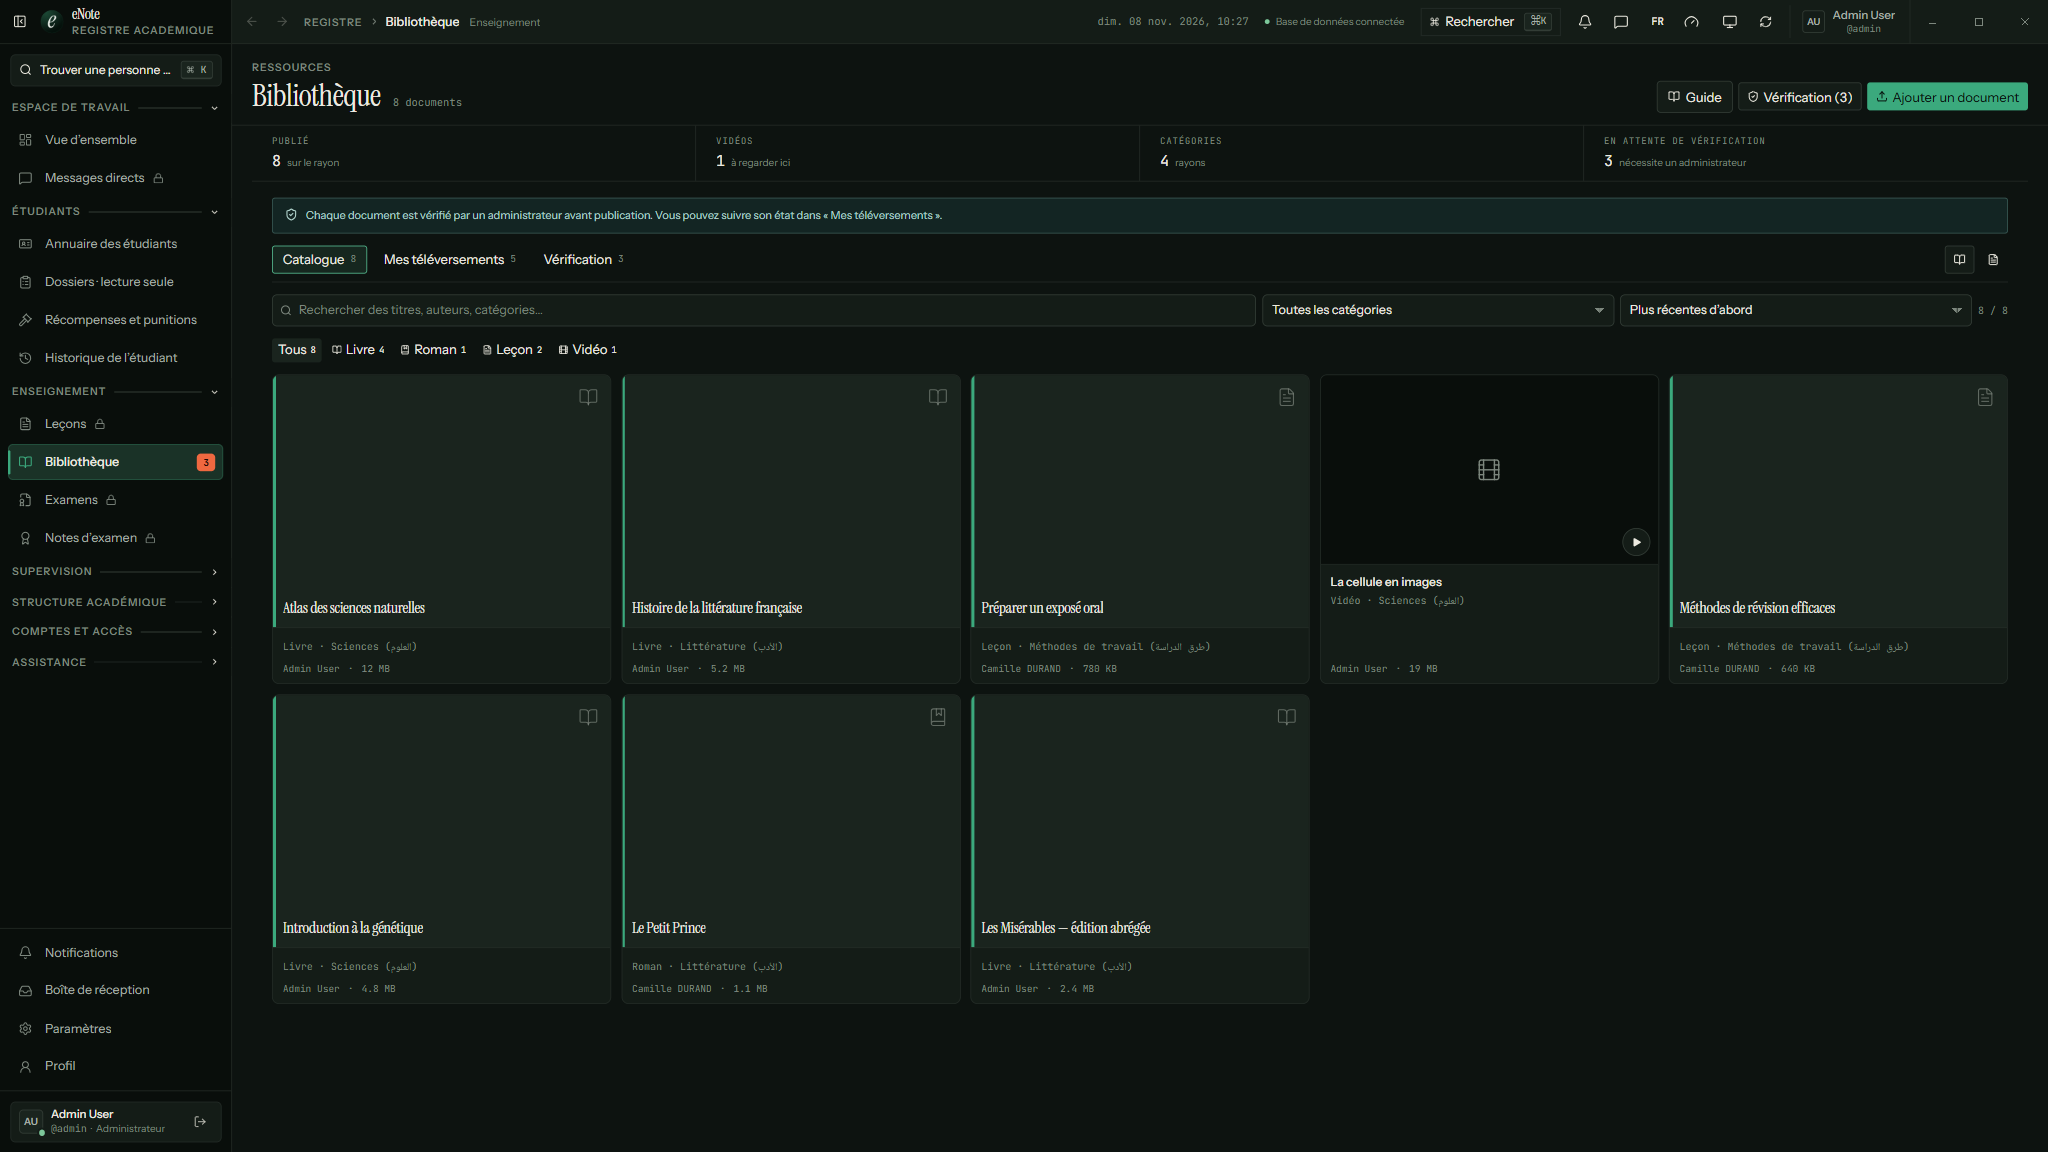
\includegraphics[width=0.85\textwidth]{images/commun_bibliotheque.png}}{\fbox{[[Capture : images/commun\_bibliotheque.png]]}}
    \caption{Catalogue de la bibliothèque documentaire}
    \label{fig:commun_bibliotheque}
\end{figure}

\subsection{Profil d'Utilisateur}
\textbf{Objectif :} consulter sa carte d'identité et tenir sa photo à jour.\par
\textbf{Accès :} pied de la barre latérale > \emph{Profil}.\par
\begin{enumerate}
    \item Lire le nom, les rôles, les coordonnées et la photo.
    \item Changer la photo avec le sélecteur natif ; l'aperçu s'affiche avant validation.
    \item Demander à l'administration la correction d'une information d'état civil.
    \item Changer le nom d'utilisateur ou le mot de passe dans \emph{Paramètres > Votre compte}.
\end{enumerate}
\textbf{Règles et contrôles :} la photo est écrite sur le partage et référencée par une clé relative.
Les informations d'identité appartiennent au dossier de la personne : les modifier depuis le profil
n'est pas proposé, car la correction doit passer par le service compétent et laisser une trace. Un
changement de mot de passe exige le mot de passe actuel.\par
\textbf{Résultat attendu :} la fiche reflète l'état du registre, et la photo apparaît dans les listes et
les conversations.

\begin{figure}[H]
    \centering
    \IfFileExists{images/commun_profil.png}{\includegraphics[width=0.85\textwidth]{images/commun_profil.png}}{\fbox{[[Capture : images/commun\_profil.png]]}}
    \caption{Profil de l'utilisateur}
    \label{fig:commun_profil}
\end{figure}

\subsection{Paramètres}
\textbf{Objectif :} régler ce qui dépend du poste, du compte, ou de l'ensemble de l'application.\par
\textbf{Accès :} pied de la barre latérale > \emph{Paramètres}.\par
\begin{enumerate}
    \item Groupe \emph{Application} : consulter \emph{Quoi de neuf} et verrouiller ou déverrouiller la
          saisie des notes.
    \item Groupe \emph{Cet ordinateur} : son des notifications, mouvement de l'interface, échelle.
    \item Groupe \emph{Notifications} : choisir les familles reçues.
    \item Groupe \emph{Votre compte} : changer le nom d'utilisateur ou le mot de passe.
    \item Groupe \emph{Administration} (administrateur) : suppression d'élève, verrou de suppression des
          absences, droits de conduite, bibliothèque (dépôts, revue, téléchargement, catégorie
          obligatoire, taille maximale, catégories), version client requise, pages verrouillées, mots de
          passe, permissions de message, testeurs bêta.
    \item Groupe \emph{Registre hérité} (administrateur et développeur) : importer un ancien dump.
\end{enumerate}
\textbf{Règles et contrôles :} chaque ligne affiche sa valeur actuelle et s'ouvre sur un dialogue ; une
option globale est enregistrée dans la base et s'applique à tous les postes, alors que le son, le
mouvement et l'échelle restent locaux. Les options globales sont vérifiées par le serveur : verrouiller
la saisie des notes ou la suppression d'une absence ne se contourne pas en appelant le service
directement. Le verrou d'absence se règle en minutes après le début de la séance ; la valeur zéro le
désactive. Les lignes réservées à un autre rôle ne sont pas affichées.\par
\textbf{Résultat attendu :} les préférences personnelles sont conservées, et les décisions collectives
sont appliquées partout.

\begin{figure}[H]
    \centering
    \IfFileExists{images/commun_parametres.png}{\includegraphics[width=0.85\textwidth]{images/commun_parametres.png}}{\fbox{[[Capture : images/commun\_parametres.png]]}}
    \caption{Page des paramètres}
    \label{fig:commun_parametres}
\end{figure}

\subsection{Palette de Commandes et Raccourcis}
\textbf{Objectif :} atteindre une page, un élève ou une action sans parcourir la barre latérale.\par
\textbf{Accès :} \texttt{Ctrl+K} ou \texttt{Cmd+K}.\par
\begin{enumerate}
    \item Ouvrir la palette et taper le début d'un nom de page, d'un élève ou d'une action.
    \item Se déplacer avec les flèches, puis valider avec \texttt{Entrée}.
    \item Dans une liste, utiliser \texttt{/} pour aller à la recherche et \texttt{Échap} pour fermer
          le volet d'inspection.
\end{enumerate}
\textbf{Règles et contrôles :} la palette indexe les routes réellement accessibles au rôle du compte,
pas la totalité de l'application. Les raccourcis de liste ne s'activent pas lorsqu'un champ de saisie a
le focus.\par
\textbf{Résultat attendu :} la destination est atteinte en deux gestes, sans connaître l'arborescence.

\begin{figure}[H]
    \centering
    \IfFileExists{images/commun_palette.png}{\includegraphics[width=0.85\textwidth]{images/commun_palette.png}}{\fbox{[[Capture : images/commun\_palette.png]]}}
    \caption{Palette de commandes}
    \label{fig:commun_palette}
\end{figure}

\subsection{Tests Bêta de l'Application}
\textbf{Objectif :} recueillir, version par version, ce qui a été testé et ce qui a échoué.\par
\textbf{Accès :} menu du compte > \emph{Tests bêta} (compte marqué testeur).\par
\begin{enumerate}
    \item Choisir la version à évaluer.
    \item Cocher les fonctionnalités testées.
    \item Pour chaque problème, indiquer la gravité et une description.
    \item Laisser un commentaire général, puis \emph{Enregistrer le rapport}.
\end{enumerate}
\textbf{Règles et contrôles :} un seul rapport est conservé par testeur et par version ; il reste
modifiable jusqu'à la validation. Seuls les comptes marqués testeurs voient la page, et le drapeau est
posé par un administrateur. Les rapports sont ensuite lus par l'administrateur et le développeur.\par
\textbf{Résultat attendu :} chaque version dispose d'un retour daté, nominatif et comparable.

\begin{figure}[H]
    \centering
    \IfFileExists{images/commun_beta.png}{\includegraphics[width=0.85\textwidth]{images/commun_beta.png}}{\fbox{[[Capture : images/commun\_beta.png]]}}
    \caption{Rapport de test bêta}
    \label{fig:commun_beta}
\end{figure}

% ================================================================
% Bloc rôle : Administrateur
% ================================================================
\section{Guide d'Utilisation d'Administrateur}
\subsection{Registre des personnes}
\textbf{Objectif :} tenir le registre des personnes, distinct des comptes de connexion, et leur
attribuer leurs rôles scolaires.\par
\textbf{Accès :} Menu > Comptes et accès > \emph{Personnes}.\par
\textbf{Prérequis :} aucun ; le registre peut être rempli avant la création des comptes.\par
\begin{enumerate}
    \item Rechercher une personne par nom, rôle ou grade, ou filtrer la liste.
    \item Utiliser \emph{Ajouter une personne} et renseigner l'identité, la photo et les coordonnées.
    \item Ouvrir la fiche pour modifier les informations, le grade, le département ou la photo.
    \item Attribuer le rôle \texttt{STUDENT} ou \texttt{TEACHER} depuis la fiche ; les rôles se
          ajoutent et se terminent un par un, avec une date de fin pour un rôle qui s'arrête.
    \item Supprimer une personne uniquement si aucun dossier ne doit être conservé.
\end{enumerate}
\textbf{Règles et contrôles :} une personne peut cumuler les rôles d'étudiant et d'enseignant ; ils sont
indépendants du rôle du compte. Le département est porté par la ligne active du rôle enseignant, pas par
la personne. La suppression d'une personne emporte ses comptes : elle n'est donc pas le moyen de retirer
un élève, qui se désactive ou se supprime depuis son dossier selon l'option globale. Toute écriture est
tracée dans le journal d'activité.\par
\textbf{Résultat attendu :} la personne apparaît dans le registre, ses rôles sont à jour et les écrans
qui la listent (répertoire, emploi du temps, examens) la proposent immédiatement.

\begin{figure}[H]
    \centering
    \IfFileExists{images/admin_personnes.png}{\includegraphics[width=0.85\textwidth]{images/admin_personnes.png}}{\fbox{[[Capture : images/admin\_personnes.png]]}}
    \caption{Registre des personnes}
    \label{fig:admin_personnes}
\end{figure}

\subsection{Création et administration des comptes}
\textbf{Objectif :} donner à chaque membre du personnel un compte de connexion dont le rôle détermine
les pages et les opérations autorisées.\par
\textbf{Accès :} Menu > Comptes et accès > \emph{Comptes}.\par
\begin{enumerate}
    \item Rechercher un compte par nom, nom d'utilisateur, courriel ou rôle, puis filtrer sur
          \emph{Actif} ou \emph{Inactif}.
    \item Utiliser \emph{Modifier} sur la ligne pour changer le nom d'utilisateur, le courriel ou le
          mot de passe ; laisser les deux champs de mot de passe vides conserve le mot de passe actuel.
    \item Choisir le rôle du compte dans la même fiche, puis \emph{Enregistrer les modifications}.
    \item Activer ou désactiver le compte avec le bouton de la ligne ; cet état est distinct du rôle.
    \item Vérifier le rôle du compte et les rôles de la personne, qui sont deux informations distinctes.
    \item Pour un mot de passe oublié, la fiche du compte suffit ; \emph{Paramètres > Administration >
          Mots de passe} permet aussi de retrouver un compte par son nom.
\end{enumerate}
\textbf{Règles et contrôles :} un compte désactivé ne peut plus se connecter, mais conserve tout ce qu'il
a produit. La fiche refuse de changer l'état ou le rôle de son propre compte : une erreur de manipulation
retirerait l'accès en cours de session. Le rôle Admin ne peut pas être retiré au dernier administrateur
actif, afin qu'un établissement ne se retrouve pas sans administrateur ; un administrateur déjà
désactivé, donc privé de connexion, ne bloque pas cette opération. Le nom d'utilisateur et le courriel
doivent rester uniques, et le nouveau mot de passe suit la politique commune (huit caractères au moins,
une majuscule, une minuscule et un chiffre). Chaque changement de nom d'utilisateur, de courriel ou de
rôle est inscrit au journal d'activité avec les valeurs avant et après ; un mot de passe remplacé n'y
figure jamais. Le serveur revérifie le rôle de l'appelant : la page est réservée aux rôles
administrateur et développeur. Un compte se rattache à une personne ; plusieurs comptes peuvent désigner
la même personne, par exemple pour un enseignant qui assure aussi une direction.\par
\textbf{Résultat attendu :} le compte peut se connecter avec le rôle prévu, et ses accès changent dès la
connexion suivante.

\begin{figure}[H]
    \centering
    \IfFileExists{images/admin_comptes.png}{\includegraphics[width=0.85\textwidth]{images/admin_comptes.png}}{\fbox{[[Capture : images/admin\_comptes.png]]}}
    \caption{Liste des comptes}
    \label{fig:admin_comptes}
\end{figure}

\subsection{Comptes suspendus}
\textbf{Objectif :} rendre l'accès à un compte verrouillé après des tentatives de connexion répétées.
\par
\textbf{Accès :} Menu > Comptes et accès > \emph{Comptes suspendus}.\par
\begin{enumerate}
    \item Rechercher le compte par nom ou nom d'utilisateur.
    \item Lire la date de suspension et son motif.
    \item Utiliser \emph{Rétablir l'accès}.
    \item Si le compte était également désactivé, le réactiver depuis la page des comptes.
\end{enumerate}
\textbf{Règles et contrôles :} cinq mots de passe erronés consécutifs suspendent le compte ; le compteur
est remis à zéro par une connexion réussie ou par un rétablissement. Une suspension est vérifiée avant
la comparaison du mot de passe : même le bon mot de passe est refusé tant que le compte est suspendu.
Le rétablissement ne réactive pas un compte désactivé, car les deux états sont indépendants. Les
connexions et les rétablissements sont enregistrés dans le journal d'activité.\par
\textbf{Résultat attendu :} l'utilisateur peut se reconnecter, et la tentative abusive reste tracée.

\begin{figure}[H]
    \centering
    \IfFileExists{images/admin_suspendus.png}{\includegraphics[width=0.85\textwidth]{images/admin_suspendus.png}}{\fbox{[[Capture : images/admin\_suspendus.png]]}}
    \caption{Comptes suspendus}
    \label{fig:admin_suspendus}
\end{figure}

\subsection{Comptes secrétaires et planificateurs}
\textbf{Objectif :} délimiter ce qu'un secrétaire ou un planificateur peut faire, et sur quelles
catégories d'enseignement.\par
\textbf{Accès :} Menu > Comptes et accès > \emph{Comptes secrétaires et planificateurs}.\par
\begin{enumerate}
    \item Sélectionner un compte dans la liste.
    \item Attribuer les catégories d'enseignement dont il est responsable.
    \item Pour un secrétaire, régler les six droits de conduite : ajouter, modifier et supprimer une
          sanction ; ajouter, modifier et supprimer une récompense.
    \item Modifier le nom d'utilisateur ou le courriel du compte si nécessaire, puis enregistrer.
\end{enumerate}
\textbf{Règles et contrôles :} un secrétaire ne voit et ne modifie que les élèves des catégories
attribuées ; un planificateur ne construit que l'emploi du temps et les groupes de ces catégories. Un
compte hors périmètre est refusé par le service, même si l'élément est visible ailleurs. Les droits de
conduite sont enregistrés par action et par entité : un secrétaire peut ajouter une sanction sans
pouvoir la supprimer. Le nom d'utilisateur doit compter au moins trois caractères et rester unique ; le
courriel doit être valide. Un compte sans fiche de personne ne peut pas porter de droits.\par
\textbf{Résultat attendu :} chaque secrétaire travaille dans son périmètre, avec des droits de conduite
conformes à la délégation accordée.

\begin{figure}[H]
    \centering
    \IfFileExists{images/admin_secretaires.png}{\includegraphics[width=0.85\textwidth]{images/admin_secretaires.png}}{\fbox{[[Capture : images/admin\_secretaires.png]]}}
    \caption{Droits et périmètre d'un compte secrétaire}
    \label{fig:admin_secretaires}
\end{figure}

\subsection{Calendrier académique}
\textbf{Objectif :} fournir à l'emploi du temps, aux examens et aux statistiques une année, des
semestres et des semaines cohérents.\par
\textbf{Accès :} Menu > Structure académique > \emph{Années académiques}.\par
\begin{enumerate}
    \item Créer une année d'études, puis ses semestres.
    \item Utiliser \emph{Générer les semaines} : choisir la date de début, la date de fin, les jours de
          week-end et l'option de remplacement des semaines existantes.
    \item Vérifier la génération : une semaine va du dimanche au samedi, et les jours fériés ou les
          semaines sans cours se retirent individuellement.
    \item Enregistrer chaque bloc ; une année sans semestre n'est pas sélectionnable ailleurs.
    \item Ne supprimer une année ou un semestre qu'avant d'y rattacher des données.
\end{enumerate}
\textbf{Règles et contrôles :} une date impossible (un 31 septembre, par exemple) est refusée, et la date
de fin doit être postérieure ou égale à la date de début. Les semaines générées sont alignées sur le
dimanche ; le week-end par défaut couvre le dimanche et le samedi, et peut être modifié. La suppression
d'une année emporte ses semestres et ses semaines : elle est donc proposée avant la saisie des séances.
Les emplois du temps, les examens et les statistiques lisent ce calendrier et ne proposent que des
périodes existantes.\par
\textbf{Résultat attendu :} les sélecteurs d'année, de semestre et de semaine des autres pages
proposent le calendrier créé, sans doublon ni semaine incomplète.

\begin{figure}[H]
    \centering
    \IfFileExists{images/admin_calendrier.png}{\includegraphics[width=0.85\textwidth]{images/admin_calendrier.png}}{\fbox{[[Capture : images/admin\_calendrier.png]]}}
    \caption{Gestion des années, semestres et semaines}
    \label{fig:admin_calendrier}
\end{figure}

\subsection{Filières, chapitres et leçons}
\textbf{Objectif :} décrire le contenu pédagogique et son poids dans la moyenne.\par
\textbf{Accès :} Menu > Structure académique > \emph{Filières}.\par
\begin{enumerate}
    \item Créer les catégories de filières, puis les filières.
    \item Ouvrir une filière pour maintenir ses chapitres et ses leçons.
    \item Renseigner le facteur de la filière pour chaque semestre : il pondère la moyenne semestrielle.
    \item Déclarer les prérequis entre filières, lorsqu'une filière en suppose une autre.
\end{enumerate}
\textbf{Règles et contrôles :} une filière utilisée par une section ou un groupe ne peut pas être
supprimée sans détacher ses dépendances. Le facteur semestriel est enregistré par filière et par
semestre ; il s'applique au calcul des moyennes et non aux notes individuelles. Les chapitres et les
leçons servent de classement aux documents ; supprimer un chapitre ne supprime pas les fichiers, qui
restent attachés à leurs leçons.\par
\textbf{Résultat attendu :} la filière est disponible dans les sections, les examens et les moyennes,
avec un poids explicite dans le calcul.

\begin{figure}[H]
    \centering
    \IfFileExists{images/admin_filieres.png}{\includegraphics[width=0.85\textwidth]{images/admin_filieres.png}}{\fbox{[[Capture : images/admin\_filieres.png]]}}
    \caption{Filières, chapitres et leçons}
    \label{fig:admin_filieres}
\end{figure}

\subsection{Sections, groupes et effectifs}
\textbf{Objectif :} constituer les sections et les groupes qui suivent les cours et passent les examens.
\par
\textbf{Accès :} Menu > Structure académique > \emph{Sections}.\par
\begin{enumerate}
    \item Créer une section et choisir sa catégorie d'enseignement.
    \item Définir les groupes d'une filière pour le semestre.
    \item Utiliser \emph{Gérer les membres} pour modifier l'effectif d'un groupe.
    \item Utiliser \emph{Groupe dynamique} pour constituer un groupe à partir d'une filière et d'un
          semestre.
\end{enumerate}
\textbf{Règles et contrôles :} supprimer une section ou un groupe détache ses étudiants au lieu de les
supprimer. Un étudiant peut être affecté à plusieurs sections, mais l'affectation courante pilote son
emploi du temps et sa place aux examens. Les groupes d'une filière sont résolus par le couple
(filière, semestre) au moment de la disposition des examens.\par
\textbf{Résultat attendu :} les listes d'étudiants des enseignants, les emplois du temps et les
répartitions d'examen reflètent les effectifs réels.

\begin{figure}[H]
    \centering
    \IfFileExists{images/admin_sections.png}{\includegraphics[width=0.85\textwidth]{images/admin_sections.png}}{\fbox{[[Capture : images/admin\_sections.png]]}}
    \caption{Sections et groupes}
    \label{fig:admin_sections}
\end{figure}

\subsection{Salles, places et registres de référence}
\textbf{Objectif :} tenir les référentiels sur lesquels reposent la planification et les formulaires.
\par
\textbf{Accès :} \emph{Paramètres > Registres}, et Menu > Structure académique > \emph{Salles}.\par
\begin{enumerate}
    \item Créer les salles avec leur code, leur capacité et leur catégorie.
    \item Générer les places d'une salle, ou les ajouter et les retirer une par une.
    \item Tenir les registres : types de séance, créneaux horaires, catégories d'enseignement,
          directions, départements, grades, types d'examen et promotions.
    \item Renseigner chaque libellé dans les trois langues ; l'anglais est obligatoire.
\end{enumerate}
\textbf{Règles et contrôles :} une salle, un type ou un grade encore utilisé ne peut pas être supprimé.
Les places conditionnent la disposition des examens : une place inexistante est refusée, et une même
place ne peut pas accueillir deux étudiants dans la même salle. Les registres alimentent les listes
déroulantes de toutes les autres pages ; une valeur ajoutée est donc immédiatement proposée.\par
\textbf{Résultat attendu :} les formulaires proposent des valeurs contrôlées, et la planification
s'appuie sur des salles dont la capacité est réelle.

\begin{figure}[H]
    \centering
    \IfFileExists{images/admin_registres.png}{\includegraphics[width=0.85\textwidth]{images/admin_registres.png}}{\fbox{[[Capture : images/admin\_registres.png]]}}
    \caption{Registres de référence et places d'une salle}
    \label{fig:admin_registres}
\end{figure}

\subsection{Examens et verrouillage des notes}
\textbf{Objectif :} superviser les examens et décider du moment où les notes ne sont plus modifiables.
\par
\textbf{Accès :} Menu > Enseignement > \emph{Examens}, et \emph{Paramètres > Application}.\par
\begin{enumerate}
    \item Vérifier les examens programmés, leur filière, leur coefficient et leur disposition.
    \item Ouvrir \emph{Paramètres > Verrouiller la saisie des notes}.
    \item Choisir \emph{Verrouillé} lorsque la campagne de notes est terminée.
    \item Consulter les notes et les moyennes pour contrôle avant la publication.
\end{enumerate}
\textbf{Règles et contrôles :} le verrou est appliqué par le serveur : un enseignant qui appelle
directement le service reçoit un refus, la page devenant seulement en lecture seule. Le verrou ne bloque
ni la programmation d'un examen, ni sa disposition, ni la consultation des moyennes. Les notes saisies
sont conservées dans un historique, ce qui permet de revenir sur une correction sans perdre la valeur
précédente.\par
\textbf{Résultat attendu :} plus aucune note ne change après la clôture, et les moyennes restent
consultables.

\begin{figure}[H]
    \centering
    \IfFileExists{images/admin_examens.png}{\includegraphics[width=0.85\textwidth]{images/admin_examens.png}}{\fbox{[[Capture : images/admin\_examens.png]]}}
    \caption{Verrouillage de la saisie des notes}
    \label{fig:admin_examens}
\end{figure}

\subsection{Statistiques et pilotage}
\textbf{Objectif :} lire l'état du registre sous forme de chiffres et de graphiques pour un semestre.\par
\textbf{Accès :} Menu > Supervision > \emph{Statistiques}.\par
\begin{enumerate}
    \item Choisir une année et un semestre.
    \item Lire les cartes de synthèse : élèves, enseignants, filières, salles, examens, séances,
          absences.
    \item Consulter les graphiques : cinq meilleurs étudiants, dix meilleures moyennes semestrielles,
          distribution des notes, effectifs par filière, absences par justification, sanctions et
          récompenses par justification, répartition par sexe.
    \item Descendre aux tableaux par filière pour le détail derrière un chiffre.
\end{enumerate}
\textbf{Règles et contrôles :} la page est réservée au rôle administrateur. Les chiffres portent sur le
semestre sélectionné, sauf les graphiques explicitement marqués « toutes périodes » (justifications des
sanctions et des récompenses). Un semestre sans données affiche un état vide explicite plutôt que des
zéros trompeurs.\par
\textbf{Résultat attendu :} une vue chiffrée et graphique du semestre, utilisable en conseil.

\begin{figure}[H]
    \centering
    \IfFileExists{images/admin_statistiques.png}{\includegraphics[width=0.85\textwidth]{images/admin_statistiques.png}}{\fbox{[[Capture : images/admin\_statistiques.png]]}}
    \caption{Tableau de bord statistique}
    \label{fig:admin_statistiques}
\end{figure}

\subsection{Journal d'activité}
\textbf{Objectif :} savoir qui a fait quoi, quand, et avec quel résultat.\par
\textbf{Accès :} Menu > Support > \emph{Journal d'activité}.\par
\begin{enumerate}
    \item Filtrer par période, acteur, action, type d'entité ou résultat.
    \item Utiliser la recherche libre pour un nom, une action ou un texte d'erreur.
    \item Parcourir les pages de vingt-cinq entrées.
    \item Exporter au format \ac{CSV} le sous-ensemble filtré.
\end{enumerate}
\textbf{Règles et contrôles :} le journal est en ajout seul : l'application refuse de modifier ou de
supprimer une entrée, y compris à un administrateur. Les entrées de plus de douze mois sont élaguées
automatiquement. L'export est plafonné pour ne pas bloquer la fenêtre, et il porte sur les filtres
actifs, non sur la seule page affichée. Les échecs de connexion y figurent avec leur motif, sans le mot
de passe essayé.\par
\textbf{Résultat attendu :} une trace exploitable pour un audit ou une investigation, sans possibilité
de réécriture.

\begin{figure}[H]
    \centering
    \IfFileExists{images/admin_journal.png}{\includegraphics[width=0.85\textwidth]{images/admin_journal.png}}{\fbox{[[Capture : images/admin\_journal.png]]}}
    \caption{Journal d'activité filtré}
    \label{fig:admin_journal}
\end{figure}

\subsection{Console de diagnostic de la base}
\textbf{Objectif :} vérifier l'état de la connexion et inspecter une table sans quitter l'application.
\par
\textbf{Accès :} Menu > Support > \emph{Base de données}.\par
\begin{enumerate}
    \item Lire l'état de la connexion et l'adresse du serveur utilisée.
    \item Choisir une table et parcourir ses colonnes et ses lignes.
    \item Exécuter une requête de lecture dans la console.
    \item Revenir à l'application ; aucune écriture n'est proposée depuis cette page.
\end{enumerate}
\textbf{Règles et contrôles :} la page est un outil de diagnostic, pas un éditeur : elle ne modifie pas
les données. La connexion vient de la configuration enregistrée ou du préréglage machine ; le mot de
passe n'est jamais affiché. Une requête lente ou une table volumineuse peut être interrompue en quittant
la page.\par
\textbf{Résultat attendu :} un diagnostic reproductible, sans accès direct au serveur PostgreSQL.

\begin{figure}[H]
    \centering
    \IfFileExists{images/admin_diagnostic.png}{\includegraphics[width=0.85\textwidth]{images/admin_diagnostic.png}}{\fbox{[[Capture : images/admin\_diagnostic.png]]}}
    \caption{Console de diagnostic de la base}
    \label{fig:admin_diagnostic}
\end{figure}

\subsection{Options globales et registre hérité}
\textbf{Objectif :} régler les décisions qui engagent l'établissement et, si nécessaire, reprendre
l'ancien registre.\par
\textbf{Accès :} \emph{Paramètres > Administration} et \emph{Paramètres > Registre hérité}.\par
\begin{enumerate}
    \item Autoriser ou interdire la suppression d'un élève.
    \item Définir les droits de conduite de chaque secrétaire.
    \item Ouvrir ou fermer les dépôts de la bibliothèque, imposer la revue, autoriser le téléchargement,
          exiger une catégorie et fixer la taille maximale ; gérer les catégories.
    \item Fixer la version client requise, verrouiller des pages, réinitialiser un mot de passe,
          autoriser les paires de rôles pour la messagerie, marquer les testeurs bêta.
    \item Pour une reprise : choisir un ancien dump, prévisualiser la correspondance, puis exécuter
          l'import dans un registre vide.
\end{enumerate}
\textbf{Règles et contrôles :} la suppression d'élève est refusée par le serveur lorsqu'elle est
interdite : le bouton disparaît, mais l'appel direct échoue aussi. Une page verrouillée reste lisible et
perd ses actions d'écriture. La réinitialisation d'un mot de passe ne renvoie jamais l'ancien mot de
passe et remet le compteur d'échecs à zéro. L'import hérité est marqué expérimental et n'écrit que dans
un registre vide, après une prévisualisation explicite.\par
\textbf{Résultat attendu :} les règles collectives sont appliquées partout, et une migration depuis
l'ancien outil reste contrôlée.

\begin{figure}[H]
    \centering
    \IfFileExists{images/admin_options.png}{\includegraphics[width=0.85\textwidth]{images/admin_options.png}}{\fbox{[[Capture : images/admin\_options.png]]}}
    \caption{Options globales de l'établissement}
    \label{fig:admin_options}
\end{figure}

\subsection{Bibliothèque : catégories, politique et revue}
\textbf{Objectif :} ouvrir ou fermer les dépôts, définir les rayons et publier les documents proposés.\par
\textbf{Accès :} Menu > Enseignement > \emph{Bibliothèque} ; \emph{Paramètres > Administration >
Bibliothèque}.\par
\begin{enumerate}
    \item Dans les paramètres, autoriser ou fermer les dépôts, puis ceux des enseignants ; imposer ou
          non la revue ; autoriser ou non le téléchargement étudiant ; exiger ou non une catégorie ;
          fixer la taille maximale d'un fichier (1 à 4~096 Mo).
    \item Ouvrir \emph{Catégories}, créer un rayon avec son code, ses libellés anglais, arabe et
          français et son ordre d'affichage ; renommer ou archiver un rayon existant.
    \item Ouvrir l'onglet \emph{Revue} : la file liste les dépôts en attente, avec les totaux du
          catalogue et les dernières lectures.
    \item Ouvrir un document, vérifier le fichier et son public, puis \emph{Publier} ou \emph{Rejeter}
          en rédigeant une note pour l'auteur.
    \item Archiver un document publié pour le retirer du catalogue sans le supprimer ; le republier
          ensuite si nécessaire.
\end{enumerate}
\textbf{Règles et contrôles :} la revue est active par défaut. Un dépôt en attente n'est visible que par
son auteur et par les bibliothécaires ; une publication le rend visible selon son public. Un rejet
conserve la note du réviseur, que l'auteur lit dans \emph{Mes dépôts} avant de corriger et de soumettre
à nouveau. Une demande de revue est notifiée aux administrateurs, et la décision est notifiée à
l'auteur. Archiver une catégorie la retire des nouveaux dépôts sans toucher aux documents déjà classés ;
un document archivé reste dans la base. Les exécutables sont refusés, la taille maximale est bornée et
chaque opération est tracée dans le journal d'activité. Le développeur, qui maintient l'installation,
dispose des mêmes droits de bibliothécaire.\par
\textbf{Résultat attendu :} le catalogue ne contient que des documents contrôlés, classés et visibles
par le public prévu.

\begin{figure}[H]
    \centering
    \IfFileExists{images/admin_bibliotheque.png}{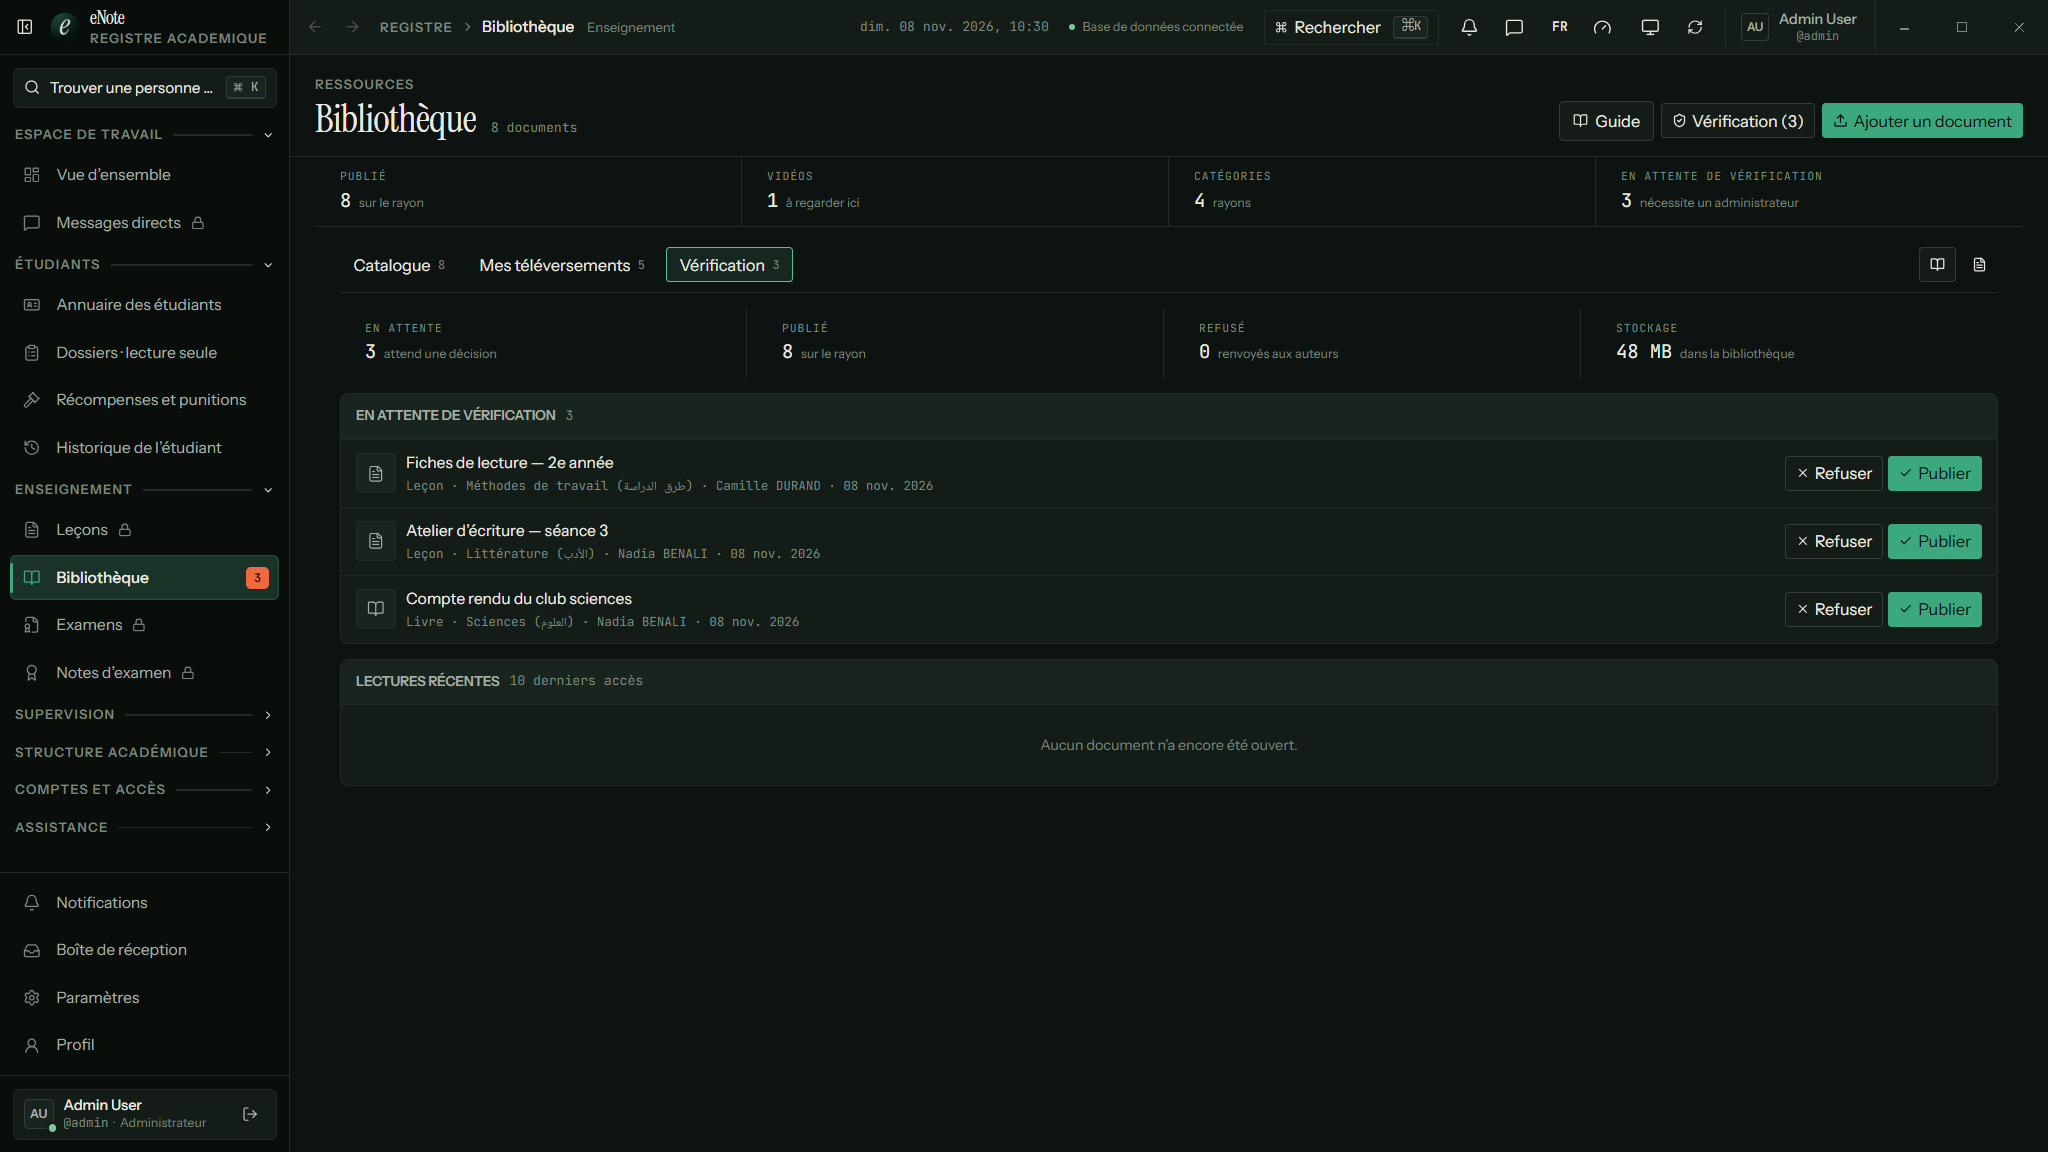
\includegraphics[width=0.85\textwidth]{images/admin_bibliotheque.png}}{\fbox{[[Capture : images/admin\_bibliotheque.png]]}}
    \caption{Revue et catégories de la bibliothèque}
    \label{fig:admin_bibliotheque}
\end{figure}

% ================================================================
% Bloc rôle : Directeur
% ================================================================
\section{Guide d'Utilisation de Directeur}
\subsection{Vue d'ensemble}
\textbf{Objectif :} savoir, en ouvrant l'application, ce qui demande une décision.\par
\textbf{Accès :} Menu > Espace de travail > \emph{Overview}.\par
\begin{enumerate}
    \item Lire la bande de chiffres : élèves, sections, assiduité, absences.
    \item Parcourir la file de travail : elle signale les élèves sans section, les examens sans notes et
          les messages non lus.
    \item Ouvrir une ligne pour arriver sur la page déjà filtrée.
    \item Consulter les séances du jour et les derniers mouvements.
\end{enumerate}
\textbf{Règles et contrôles :} chaque chiffre est un lien vers la liste qu'il décrit, et le filtre arrive
sous forme de pastille visible, de sorte que la page explique pourquoi elle est filtrée. Un
établissement sans élèves affiche les étapes de mise en place dans l'ordre requis, au lieu de zéros.\par
\textbf{Résultat attendu :} le directeur choisit sa prochaine action sans parcourir les menus.

\begin{figure}[H]
    \centering
    \IfFileExists{images/directeur_overview.png}{\includegraphics[width=0.85\textwidth]{images/directeur_overview.png}}{\fbox{[[Capture : images/directeur\_overview.png]]}}
    \caption{Vue d'ensemble du directeur}
    \label{fig:directeur_overview}
\end{figure}

\subsection{Consultation d'un dossier d'élève}
\textbf{Objectif :} lire le dossier complet d'un élève sans pouvoir le modifier.\par
\textbf{Accès :} Menu > Élèves > \emph{Dossiers (lecture seule)}, ou \emph{Répertoire des élèves}.\par
\begin{enumerate}
    \item Rechercher l'élève par nom ou par référence.
    \item Sélectionner la ligne : le volet d'inspection s'ouvre à droite.
    \item Parcourir les onglets Identité, Santé et corps, Documents et scolarité, Famille, Loisirs,
          Contacts d'urgence et Uniformes.
    \item Utiliser \emph{Ouvrir le dossier complet} pour la vue en trois colonnes.
    \item Consulter l'historique des affectations et des changements de section.
\end{enumerate}
\textbf{Règles et contrôles :} aucune action d'écriture n'est proposée : le rôle directeur ne peut ni
inscrire, ni corriger, ni supprimer. Les corrections relèvent de l'administration ou du secrétaire de la
catégorie. Les pièces sensibles (santé, famille) sont affichées parce que la consultation fait partie
de la fonction, mais chaque ouverture de dossier est tracée dans le journal d'activité.\par
\textbf{Résultat attendu :} le dossier est consultable en lecture seule, sans risque de modification
accidentelle.

\begin{figure}[H]
    \centering
    \IfFileExists{images/directeur_dossier.png}{\includegraphics[width=0.85\textwidth]{images/directeur_dossier.png}}{\fbox{[[Capture : images/directeur\_dossier.png]]}}
    \caption{Volet d'inspection d'un dossier d'élève}
    \label{fig:directeur_dossier}
\end{figure}

\subsection{Enregistrements de séances et commentaires}
\textbf{Objectif :} vérifier, pour une semaine, ce que les enseignants ont enregistré, et laisser une
appréciation de direction.\par
\textbf{Accès :} Menu > Supervision > \emph{Enregistrements de séances}.\par
\begin{enumerate}
    \item Choisir l'année, le semestre et la semaine.
    \item Filtrer par jour, filière ou enseignant.
    \item Ouvrir une séance pour lire ses absences et ses observations, et vérifier qu'elle a bien été
          tenue.
    \item Commenter une absence ou une observation depuis sa ligne.
    \item Utiliser \emph{Exporter le rapport} pour imprimer la semaine.
\end{enumerate}
\textbf{Règles et contrôles :} la page ne modifie rien : les présences et les observations sont saisies
par les enseignants. Le commentaire est réservé au rôle directeur, et tous les directeurs partagent le
même fil : un commentaire n'est pas privé. Un administrateur lit les mêmes enregistrements mais ne
commente pas. Une séance sans enregistrement apparaît comme non renseignée, pas comme absence
d'élèves.\par
\textbf{Résultat attendu :} la semaine est vérifiable séance par séance, et une appréciation de direction
reste attachée à l'enregistrement.

\begin{figure}[H]
    \centering
    \IfFileExists{images/directeur_seances.png}{\includegraphics[width=0.85\textwidth]{images/directeur_seances.png}}{\fbox{[[Capture : images/directeur\_seances.png]]}}
    \caption{Enregistrements d'une semaine}
    \label{fig:directeur_seances}
\end{figure}

\subsection{Assiduité des enseignants}
\textbf{Objectif :} repérer les séances qui n'ont pas été tenues et suivre le taux de réalisation.\par
\textbf{Accès :} Menu > Supervision > \emph{Assiduité des enseignants}.\par
\begin{enumerate}
    \item Choisir une période : sept, trente ou quatre-vingt-dix derniers jours, ou deux dates.
    \item Filtrer par enseignant, ou laisser la liste complète.
    \item Lire la marque de chaque séance : tenue, manquée ou non encore décidée.
    \item Utiliser le taux par enseignant pour relancer celui qui accumule les séances manquées.
\end{enumerate}
\textbf{Règles et contrôles :} une séance compte comme tenue dès qu'elle possède un enregistrement :
une absence, une observation ou une confirmation « tenue, rien à signaler ». Elle compte comme manquée
lorsque son créneau est terminé sans aucun enregistrement ; une séance qui n'est pas encore finie
n'entre dans aucune colonne, afin qu'un cours de l'après-midi ne soit pas compté comme manqué le matin.
La période est inclusive, et une date de début postérieure à la date de fin est refusée.\par
\textbf{Résultat attendu :} une vue par période des séances non tenues, sans modification possible des
données.

\begin{figure}[H]
    \centering
    \IfFileExists{images/directeur_assiduite.png}{\includegraphics[width=0.85\textwidth]{images/directeur_assiduite.png}}{\fbox{[[Capture : images/directeur\_assiduite.png]]}}
    \caption{Rapport d'assiduité des enseignants}
    \label{fig:directeur_assiduite}
\end{figure}

\subsection{Historique d'un élève}
\textbf{Objectif :} reconstituer le parcours d'un élève avant une décision.\par
\textbf{Accès :} Menu > Élèves > \emph{Historique de l'élève}.\par
\begin{enumerate}
    \item Choisir un élève dans la liste, en filtrant au besoin par section, filière ou niveau.
    \item Lire les graphiques : tendance des absences, répartition des observations.
    \item Filtrer les enregistrements par justification, motif, filière ou enseignant.
    \item Descendre au tableau des enregistrements individuels, avec leur date et leur auteur.
\end{enumerate}
\textbf{Règles et contrôles :} les filtres portent sur l'historique de l'élève choisi et non sur la liste
des élèves ; changer d'élève réinitialise les filtres dépendants pour éviter une vue incohérente. La
page est en lecture seule : elle sert à préparer une décision, pas à la consigner.\par
\textbf{Résultat attendu :} une synthèse visuelle et un tableau détaillé, utilisables en conseil de
discipline.

\begin{figure}[H]
    \centering
    \IfFileExists{images/directeur_historique.png}{\includegraphics[width=0.85\textwidth]{images/directeur_historique.png}}{\fbox{[[Capture : images/directeur\_historique.png]]}}
    \caption{Historique des absences et observations}
    \label{fig:directeur_historique}
\end{figure}

\subsection{Historique global}
\textbf{Objectif :} comparer les sections et les filières sur une période, sans partir d'un élève.\par
\textbf{Accès :} Menu > Supervision > \emph{Historique global}.\par
\begin{enumerate}
    \item Définir la période et le type d'enregistrement.
    \item Filtrer par filière et par section.
    \item Lire les graphiques de tendance, puis le tableau des enregistrements.
    \item Réinitialiser les filtres pour revenir à la période complète.
\end{enumerate}
\textbf{Règles et contrôles :} la page est une vue de supervision : rien n'y est édité. Un filtre trop
étroit peut produire un tableau vide ; l'état vide le dit explicitement et propose de réinitialiser.
Les totaux portent sur les enregistrements filtrés, pas sur l'ensemble du registre.\par
\textbf{Résultat attendu :} une comparaison entre sections et filières, appuyée sur les mêmes
enregistrements que les pages individuelles.

\begin{figure}[H]
    \centering
    \IfFileExists{images/directeur_global.png}{\includegraphics[width=0.85\textwidth]{images/directeur_global.png}}{\fbox{[[Capture : images/directeur\_global.png]]}}
    \caption{Historique global}
    \label{fig:directeur_global}
\end{figure}

\subsection{Bibliothèque documentaire}
\textbf{Objectif :} superviser ce qui est publié et vérifier que le catalogue correspond aux besoins
pédagogiques.\par
\textbf{Accès :} Menu > Enseignement > \emph{Bibliothèque}.\par
\begin{enumerate}
    \item Parcourir le catalogue et filtrer par type, catégorie ou auteur.
    \item Ouvrir un document pour lire sa fiche, son public et son historique de publication.
    \item Consulter le nombre de lectures et de téléchargements.
    \item Signaler à l'administration un document à retirer ou une catégorie à compléter.
\end{enumerate}
\textbf{Règles et contrôles :} le directeur voit tous les documents, y compris ceux qui ne sont pas
publiés, mais la page reste en lecture seule : il ne publie, ne rejette, ne modifie et ne supprime
aucun document. La revue et les catégories appartiennent à l'administrateur ou au développeur. Les
compteurs de lecture ne constituent pas une évaluation pédagogique et ne sont pas exportés dans le
rapport individuel.\par
\textbf{Résultat attendu :} la direction sait ce que l'établissement met à disposition, sans se
substituer au bibliothécaire.

\subsection{Génération du rapport individuel PDF}
\textbf{Objectif :} produire un document officiel remis à l'élève ou versé à son dossier.\par
\textbf{Accès :} dossier de l'élève > \emph{Exporter le rapport (PDF)}.\par
\begin{enumerate}
    \item Choisir les rubriques à inclure : identité, scolarité, absences, observations, conduite.
    \item Choisir la langue du document : anglais, arabe ou français.
    \item Lancer la génération ; le document est construit par Chromium avec les polices embarquées.
    \item Choisir l'emplacement d'enregistrement dans le dialogue natif.
    \item Ouvrir le fichier pour vérifier la mise en page, notamment en arabe.
\end{enumerate}
\textbf{Règles et contrôles :} le rapport est réservé au rôle directeur. Les polices sont embarquées :
le fichier est identique sur un poste qui n'a aucune police arabe installée. Le nom du fichier reprend
l'identifiant de la personne, son nom et la langue ; un nom invalide pour le système est nettoyé. Un
poste sans lecteur \ac{PDF} peut toujours enregistrer le fichier et l'ouvrir ailleurs.\par
\textbf{Résultat attendu :} un fichier autonome, lisible hors ligne, conforme à la langue choisie.

\begin{figure}[H]
    \centering
    \IfFileExists{images/directeur_pdf.png}{\includegraphics[width=0.85\textwidth]{images/directeur_pdf.png}}{\fbox{[[Capture : images/directeur\_pdf.png]]}}
    \caption{Rapport individuel au format PDF}
    \label{fig:directeur_pdf}
\end{figure}

% ================================================================
% Bloc rôle : Secrétaire
% ================================================================
\section{Guide d'Utilisation de Secrétaire}
\subsection{Périmètre des catégories}
\textbf{Objectif :} comprendre ce que le compte peut voir et modifier avant de commencer.\par
\textbf{Accès :} Menu > Élèves > \emph{Répertoire des élèves}.\par
\begin{enumerate}
    \item Lire la bandeau de portée en haut de la liste : il nomme les catégories autorisées.
    \item Vérifier qu'un élève recherché apparaît ; un élève hors périmètre n'est pas listé.
    \item Ouvrir un élève autorisé : les actions d'écriture sont proposées.
    \item Si une catégorie manque, demander à l'administrateur de l'attribuer au compte.
\end{enumerate}
\textbf{Règles et contrôles :} le périmètre est appliqué par le serveur à chaque lecture et à chaque
écriture. Un identifiant d'élève hors périmètre appelé directement est refusé, même si l'interface ne
l'a jamais affiché. Le bandeau reste visible pour que l'utilisateur sache pourquoi un élève est absent
de la liste, plutôt que de conclure à une erreur.\par
\textbf{Résultat attendu :} le secrétaire travaille dans un périmètre explicite, sans risque d'écrire
hors de sa responsabilité.

\begin{figure}[H]
    \centering
    \IfFileExists{images/secretariat_portee.png}{\includegraphics[width=0.85\textwidth]{images/secretariat_portee.png}}{\fbox{[[Capture : images/secretariat\_portee.png]]}}
    \caption{Bandeau de portée du secrétaire}
    \label{fig:secretariat_portee}
\end{figure}

\subsection{Inscription d'un nouvel élève}
\textbf{Objectif :} créer le dossier complet d'un élève entrant.\par
\textbf{Accès :} Menu > Élèves > \emph{Répertoire des élèves} > \emph{Inscrire un élève}.\par
\textbf{Prérequis :} la catégorie d'enseignement de l'élève doit figurer parmi celles du compte ; les
listes de référence (grades, santé, professions, loisirs) doivent être renseignées.\par
\begin{enumerate}
    \item Onglet \emph{Identité} : identifiant, noms en écriture latine et arabe, date de naissance,
          sexe et grade. L'identifiant peut être saisi manuellement et doit être unique.
    \item Onglet \emph{Santé et corps} : groupe sanguin, statut de santé, taille, poids, port du
          collier militaire, numéro d'armée.
    \item Onglet \emph{Scolarité} : numéro national, acte de naissance, compte postal, série
          d'ordinateur, carte d'assurance, carte militaire, numéro de casque, baccalauréat, certificat
          scolaire, niveau académique, spécialité, moyenne académique et source de recrutement.
    \item Onglet \emph{Famille} : noms des parents dans les deux écritures, professions, nombre de
          frères et s\oe{}urs, rang dans la fratrie, situation des parents et statut d'orphelin.
    \item Onglets \emph{Loisirs}, \emph{Contacts d'urgence} et \emph{Uniformes et adresse} : compléter
          les informations disponibles.
    \item Onglet \emph{Section} : affecter une section, puis enregistrer.
\end{enumerate}
\textbf{Règles et contrôles :} le prénom et le nom sont obligatoires. Les identifiants numériques
n'acceptent que des chiffres et peuvent rester vides, mais un identifiant déjà utilisé est refusé. La
moyenne académique doit être comprise entre 0 et 20 ; la taille et le poids sont bornés par le service.
Pour un parent, les deux noms doivent être renseignés ensemble ou laissés vides ensemble. La section
proposée est limitée aux catégories du compte. Un dossier incomplet peut être enregistré, mais la
colonne de complétude le signale.\par
\textbf{Résultat attendu :} l'élève apparaît dans le répertoire, son dossier est consultable par les
rôles habilités et il peut être inscrit aux examens.

\begin{figure}[H]
    \centering
    \IfFileExists{images/secretariat_inscription.png}{\includegraphics[width=0.85\textwidth]{images/secretariat_inscription.png}}{\fbox{[[Capture : images/secretariat\_inscription.png]]}}
    \caption{Formulaire d'inscription d'un élève}
    \label{fig:secretariat_inscription}
\end{figure}

\subsection{Mise à jour et complétude d'un dossier}
\textbf{Objectif :} corriger une information, compléter un dossier incomplet ou changer la photo.\par
\textbf{Accès :} \emph{Répertoire des élèves} > sélectionner l'élève > \emph{Modifier}.\par
\begin{enumerate}
    \item Repérer la colonne de complétude : elle indique le nombre d'informations manquantes.
    \item Ouvrir l'onglet concerné et corriger les champs.
    \item Changer la photo avec le sélecteur natif ; l'aperçu s'affiche avant validation.
    \item Enregistrer, puis vérifier la fiche et l'historique des modifications.
\end{enumerate}
\textbf{Règles et contrôles :} les identifiants sont vérifiés en direct pendant la saisie, ce qui évite
de découvrir un doublon à l'enregistrement. Retirer une photo supprime le fichier du partage : ce n'est
donc pas une action en un clic, et l'interface demande confirmation. Les corrections sont tracées dans
l'historique de la personne, avec l'ancienne et la nouvelle valeur. Un élève hors périmètre n'ouvre
pas le formulaire. Une saisie interrompue — fermeture de la fenêtre, coupure du poste ou du serveur —
est conservée quatorze jours sur l'ordinateur, par formulaire et par compte, puis proposée à la
réouverture ; l'application ne la réapplique jamais d'elle-même et l'efface dès que l'enregistrement
réussit.\par
\textbf{Résultat attendu :} les corrections sont immédiatement visibles pour tous les services, et
l'historique conserve la valeur précédente.

\begin{figure}[H]
    \centering
    \IfFileExists{images/secretariat_dossier.png}{\includegraphics[width=0.85\textwidth]{images/secretariat_dossier.png}}{\fbox{[[Capture : images/secretariat\_dossier.png]]}}
    \caption{Onglets du dossier de l'élève}
    \label{fig:secretariat_dossier}
\end{figure}

\subsection{Recherche, filtres et export du répertoire}
\textbf{Objectif :} retrouver rapidement un élève ou un ensemble d'élèves, puis exporter la vue.\par
\textbf{Accès :} \emph{Répertoire des élèves} > barre d'outils.\par
\begin{enumerate}
    \item Taper un nom ou un identifiant dans la recherche.
    \item Filtrer par catégorie, section ou état du dossier (complet, incomplet, sans section).
    \item Trier par nom, identifiant, date de naissance, catégorie ou section.
    \item Utiliser \emph{Exporter CSV} pour écrire les lignes affichées.
\end{enumerate}
\textbf{Règles et contrôles :} les filtres actifs restent visibles sous forme de pastilles, ce qui évite
une liste filtrée sans explication. La recherche et le tri sont conservés lorsqu'on ouvre un élève puis
qu'on revient. L'export porte sur la vue courante, pas sur l'ensemble du registre, et le nom du fichier
est daté. La colonne de complétude n'est proposée qu'aux rôles qui ont la charge de compléter les
dossiers.\par
\textbf{Résultat attendu :} la liste utile est obtenue en quelques secondes et peut être transmise au
service demandeur.

\begin{figure}[H]
    \centering
    \IfFileExists{images/secretariat_repertoire.png}{\includegraphics[width=0.85\textwidth]{images/secretariat_repertoire.png}}{\fbox{[[Capture : images/secretariat\_repertoire.png]]}}
    \caption{Recherche et filtres du répertoire}
    \label{fig:secretariat_repertoire}
\end{figure}

\subsection{Affectation à une section}
\textbf{Objectif :} placer un élève, ou un groupe d'élèves, dans la section qui correspond à son
parcours.\par
\textbf{Accès :} \emph{Répertoire des élèves} > \emph{Affecter une section}.\par
\begin{enumerate}
    \item Sélectionner un ou plusieurs élèves.
    \item Choisir la section de destination, limitée aux catégories autorisées.
    \item Lire le récapitulatif : \emph{Cette action déplace N élèves de la section X vers la section
          Y.}
    \item Confirmer ; l'ancienne affectation reste dans l'historique.
\end{enumerate}
\textbf{Règles et contrôles :} une affectation remplace l'affectation courante mais n'efface pas
l'historique : la date de début et de fin de chaque passage est conservée. Retirer un élève d'une
section est une action distincte, qui le laisse inscrit mais sans section ; il apparaît alors dans la
file de travail « élèves sans section ». L'affectation est refusée si la section n'appartient pas au
périmètre du compte.\par
\textbf{Résultat attendu :} l'élève figure dans la nouvelle section, son historique d'affectation est
mis à jour et les listes des enseignants suivent.

\begin{figure}[H]
    \centering
    \IfFileExists{images/secretariat_section.png}{\includegraphics[width=0.85\textwidth]{images/secretariat_section.png}}{\fbox{[[Capture : images/secretariat\_section.png]]}}
    \caption{Affectation d'élèves à une section}
    \label{fig:secretariat_section}
\end{figure}

\subsection{Récompenses et sanctions}
\textbf{Objectif :} consigner un encouragement ou une sanction, individuellement ou pour un groupe.\par
\textbf{Accès :} Menu > Élèves > \emph{Récompenses et sanctions}.\par
\begin{enumerate}
    \item Rechercher l'élève ; seuls les élèves des catégories du compte sont proposés.
    \item Choisir \emph{Récompenses} ou \emph{Sanctions}, puis \emph{Nouvelle entrée}.
    \item Choisir le type et la justification, la date de début, la durée en jours et une note.
    \item Pour un groupe, basculer sur l'onglet collectif, ajouter les élèves puis appliquer.
    \item Pour modifier ou supprimer une entrée, ouvrir le panneau de l'élève.
\end{enumerate}
\textbf{Règles et contrôles :} le type et la justification sont obligatoires. Une sanction ou une
récompense planifiée exige une date de début valide et une durée en jours entiers, au moins égale à un.
Les six droits de conduite sont vérifiés à chaque action : ajouter, modifier et supprimer sont
indépendants pour les sanctions et pour les récompenses. Une action collective exige au moins un élève
sélectionné. Les entrées sont horodatées et signées par le compte qui les a créées ; une correction
conserve l'auteur d'origine dans l'historique.\par
\textbf{Résultat attendu :} l'entrée est enregistrée avec son auteur et sa date, et apparaît dans
l'historique de l'élève et dans les rapports du directeur.

\begin{figure}[H]
    \centering
    \IfFileExists{images/secretariat_conduite.png}{\includegraphics[width=0.85\textwidth]{images/secretariat_conduite.png}}{\fbox{[[Capture : images/secretariat\_conduite.png]]}}
    \caption{Récompenses et sanctions d'un élève}
    \label{fig:secretariat_conduite}
\end{figure}

\subsection{Photo et pièces du dossier}
\textbf{Objectif :} tenir à jour la photo et les pièces qui identifient l'élève.\par
\textbf{Accès :} dossier de l'élève > photo, et onglet \emph{Uniformes et adresse}.\par
\begin{enumerate}
    \item Choisir la photo depuis le dialogue natif ; l'aperçu s'affiche avant validation.
    \item Vérifier le cadrage et le poids du fichier, puis enregistrer.
    \item Renseigner l'adresse : pays, wilaya, daïra, commune et rue, dans les deux écritures.
    \item Compléter les uniformes (tenue de combat, tenue de parade) lorsque le dossier le prévoit.
\end{enumerate}
\textbf{Règles et contrôles :} la photo est écrite sur le partage et référencée par une clé relative ;
elle n'est jamais stockée dans la base. Remplacer une photo écrit un nouveau fichier et supprime
l'ancien, ce qui évite l'accumulation. Les listes d'adresse sont dépendantes : changer de pays recharge
les wilayas, changer de wilaya recharge les daïras. Un élève étranger n'a pas les mêmes champs
d'adresse, et l'onglet des contacts d'urgence est adapté en conséquence.\par
\textbf{Résultat attendu :} la photo et l'adresse sont visibles depuis tous les postes, et les
formulaires proposent des valeurs cohérentes.

\begin{figure}[H]
    \centering
    \IfFileExists{images/secretariat_documents.png}{\includegraphics[width=0.85\textwidth]{images/secretariat_documents.png}}{\fbox{[[Capture : images/secretariat\_documents.png]]}}
    \caption{Photo, adresse et uniformes}
    \label{fig:secretariat_documents}
\end{figure}

% ================================================================
% Bloc rôle : Enseignant
% ================================================================
\section{Guide d'Utilisation d'Enseignant}
\subsection{Emploi du temps et liste des étudiants}
\textbf{Objectif :} connaître ses séances de la semaine, leurs salles et leurs groupes.\par
\textbf{Accès :} Menu > Enseignement > \emph{Mon emploi du temps}.\par
\begin{enumerate}
    \item Choisir la semaine en haut de la page.
    \item Lire la grille : type de séance, salle, groupe et horaire.
    \item Ouvrir une séance pour afficher les élèves attendus.
    \item Utiliser la page pour confirmer une séance tenue.
\end{enumerate}
\textbf{Règles et contrôles :} l'emploi du temps est en lecture seule pour l'enseignant : les
déplacements relèvent du planificateur ou de l'administrateur. Une séance supprimée ou déplacée signale le changement par une notification, et une séance
nouvellement attribuée en produit une également : la grille seule ne l'annonce pas. La liste des
étudiants vient de l'affectation de section, elle n'est pas saisie par l'enseignant.\par
\textbf{Résultat attendu :} l'enseignant dispose de son programme à jour, y compris après une
modification faite par le planificateur.

\begin{figure}[H]
    \centering
    \IfFileExists{images/enseignant_emploi.png}{\includegraphics[width=0.85\textwidth]{images/enseignant_emploi.png}}{\fbox{[[Capture : images/enseignant\_emploi.png]]}}
    \caption{Emploi du temps de l'enseignant}
    \label{fig:enseignant_emploi}
\end{figure}

\subsection{Faire l'appel}
\textbf{Objectif :} enregistrer les présences et les absences d'une séance.\par
\textbf{Accès :} Menu > Enseignement > \emph{Présences} (la page s'ouvre automatiquement au début d'une
séance).\par
\begin{enumerate}
    \item Rechercher un élève dans la liste, puis le marquer absent.
    \item Choisir la justification : non justifiée par défaut, ou une justification de la liste.
    \item Ajouter une note si l'absence demande un contexte.
    \item Répéter pour chaque absence, puis enregistrer ; la ligne est écrite immédiatement.
    \item Pour retirer une absence, utiliser \emph{Présent} sur la ligne ; le bouton reste inactif
          pendant le délai de verrouillage fixé par l'administrateur, le cas échéant.
    \item Utiliser \emph{Tenue, rien à signaler} si la séance s'est déroulée normalement.
\end{enumerate}
\textbf{Règles et contrôles :} la page vérifie l'horloge toutes les quinze secondes et ouvre la séance
en cours sans intervention. Une absence est écrite immédiatement, mais sa justification peut être
corrigée plus tard. L'administrateur peut interdire la suppression d'une absence pendant les premières
minutes de la séance : le bouton \emph{Présent} est alors désactivé, et le serveur refuse la suppression
même si la demande est envoyée autrement. Le verrou ne s'applique ni à l'administrateur ni au
développeur. La confirmation « tenue, rien à signaler » crée l'enregistrement qui distingue une
séance sans incident d'une séance non renseignée. Un élève absent ne peut pas recevoir d'observation
pour la même séance.\par
\textbf{Résultat attendu :} l'absence est enregistrée avec la séance, l'élève et l'enseignant, et le
directeur la retrouve dans ses notifications et ses enregistrements.

\begin{figure}[H]
    \centering
    \IfFileExists{images/enseignant_appel.png}{\includegraphics[width=0.85\textwidth]{images/enseignant_appel.png}}{\fbox{[[Capture : images/enseignant\_appel.png]]}}
    \caption{Feuille de présence d'une séance}
    \label{fig:enseignant_appel}
\end{figure}

\subsection{Consigner une observation}
\textbf{Objectif :} noter un comportement, une difficulté ou un fait marquant pendant une séance.\par
\textbf{Accès :} Menu > Enseignement > \emph{Observations}.\par
\begin{enumerate}
    \item Choisir la section et la séance.
    \item Rechercher l'élève dans la liste ; les présents et les absents sont distingués.
    \item Utiliser \emph{Nouvelle observation}, choisir le motif et rédiger la note.
    \item Enregistrer, puis vérifier l'entrée dans la liste.
\end{enumerate}
\textbf{Règles et contrôles :} un élève absent ne peut pas recevoir d'observation pour cette séance : la
ligne est désactivée et le service refuse l'écriture. Le motif vient d'un registre administré, ce qui
permet de comparer les observations entre classes. Une entrée saisie par erreur peut être supprimée ;
la suppression est elle-même enregistrée. Les compteurs de présents et d'absents sont recalculés à
partir de la liste réelle.\par
\textbf{Résultat attendu :} l'observation est visible par le directeur, versée à l'historique de
l'élève et signalée dans les notifications.

\begin{figure}[H]
    \centering
    \IfFileExists{images/enseignant_observation.png}{\includegraphics[width=0.85\textwidth]{images/enseignant_observation.png}}{\fbox{[[Capture : images/enseignant\_observation.png]]}}
    \caption{Saisie d'une observation}
    \label{fig:enseignant_observation}
\end{figure}

\subsection{Saisie des notes d'examen}
\textbf{Objectif :} renseigner les notes d'un examen et laisser le serveur calculer les moyennes.\par
\textbf{Accès :} Menu > Enseignement > \emph{Notes d'examen}.\par
\begin{enumerate}
    \item Choisir l'examen dans la liste de ceux des filières enseignées.
    \item Saisir la note de chaque étudiant ligne par ligne.
    \item Laisser vide une note non disponible : elle est exclue de la moyenne plutôt que comptée
          comme zéro.
    \item Appuyer sur \emph{Enregistrer les notes}.
\end{enumerate}
\textbf{Règles et contrôles :} une note doit être un nombre entre 0 et 20 ; une valeur hors bornes est
refusée avec le message correspondant. Un enregistrement sans aucune note est refusé, et vider
explicitement une note est une action distincte de l'absence de saisie. L'enseignant ne peut saisir que
les examens des filières qu'il enseigne. Si l'administrateur a verrouillé la saisie, la page est en
lecture seule et le service refuse l'écriture. Chaque changement conserve la valeur précédente dans
l'historique des notes. Une saisie interrompue est conservée sur le poste, pour cet examen et ce
compte, pendant quatorze jours : à la réouverture, la page propose de restaurer ou d'abandonner les
notes non enregistrées, sans jamais les réappliquer d'elle-même.\par
\textbf{Résultat attendu :} les notes sont enregistrées avec leur historique, les moyennes suivent les
coefficients et la page reste en lecture seule lorsque la campagne est close.

\begin{figure}[H]
    \centering
    \IfFileExists{images/enseignant_notes.png}{\includegraphics[width=0.85\textwidth]{images/enseignant_notes.png}}{\fbox{[[Capture : images/enseignant\_notes.png]]}}
    \caption{Saisie des notes d'un examen}
    \label{fig:enseignant_notes}
\end{figure}

\subsection{Publication de supports de cours}
\textbf{Objectif :} mettre à disposition des étudiants les diapositives, polycopiés, images et
enregistrements d'une leçon.\par
\textbf{Accès :} Menu > Enseignement > \emph{Leçons}.\par
\begin{enumerate}
    \item Ouvrir la leçon concernée, ou la créer si elle n'existe pas.
    \item Utiliser \emph{Ajouter des fichiers} et choisir les fichiers sur le poste.
    \item Renseigner le titre, le type et la visibilité du document.
    \item Vérifier que le fichier apparaît et s'ouvre depuis la page.
\end{enumerate}
\textbf{Règles et contrôles :} les fichiers sont copiés sur le partage et référencés par une clé
relative ; l'interface ne reçoit jamais un chemin local. Une vidéo est lue dans la page, avec une image
extraite de l'enregistrement en vignette ; les autres formats s'ouvrent ou se téléchargent. Supprimer un
fichier le retire pour tous les étudiants, pas seulement pour l'enseignant. La base ne stocke pas le
contenu : une sauvegarde de la base ne sauvegarde pas les fichiers, d'où la nécessité de sauvegarder
aussi le partage.\par
\textbf{Résultat attendu :} les étudiants voient les supports à leur prochaine ouverture de la leçon,
et les vidéos se lisent directement dans la page.

\begin{figure}[H]
    \centering
    \IfFileExists{images/enseignant_lecons.png}{\includegraphics[width=0.85\textwidth]{images/enseignant_lecons.png}}{\fbox{[[Capture : images/enseignant\_lecons.png]]}}
    \caption{Supports d'une leçon}
    \label{fig:enseignant_lecons}
\end{figure}

\subsection{Déposer un document dans la bibliothèque}
\textbf{Objectif :} partager un livre, un roman, une leçon ou une vidéo avec l'établissement, hors du
support d'une leçon.\par
\textbf{Accès :} Menu > Enseignement > \emph{Bibliothèque} > \emph{Ajouter un document}.\par
\begin{enumerate}
    \item Choisir le fichier sur le poste ; un fichier vidéo est reconnu comme vidéo.
    \item Renseigner le titre, la description, la catégorie et le public (tous, enseignants ou
          étudiants).
    \item Soumettre le document, puis suivre son état dans \emph{Mes dépôts}.
    \item Tant qu'il n'est pas publié, le modifier ou le retirer ; après un rejet, lire la note du
          réviseur, corriger le fichier ou la fiche, puis soumettre à nouveau.
\end{enumerate}
\textbf{Règles et contrôles :} l'administration peut fermer les dépôts ou réserver l'ajout aux
administrateurs ; dans ce cas le bouton disparaît et le service refuse l'appel. Quand la revue est
active, un dépôt reste en attente et n'est visible ni des étudiants ni des autres enseignants. Le
fichier est copié sur le partage, la base ne garde qu'une clé relative, et un exécutable est refusé. La
taille maximale et l'obligation de catégorie sont fixées dans les paramètres.\par
\textbf{Résultat attendu :} le document rejoint le catalogue après validation, avec la fiche et le
public choisis par son auteur.

\begin{figure}[H]
    \centering
    \IfFileExists{images/enseignant_bibliotheque.png}{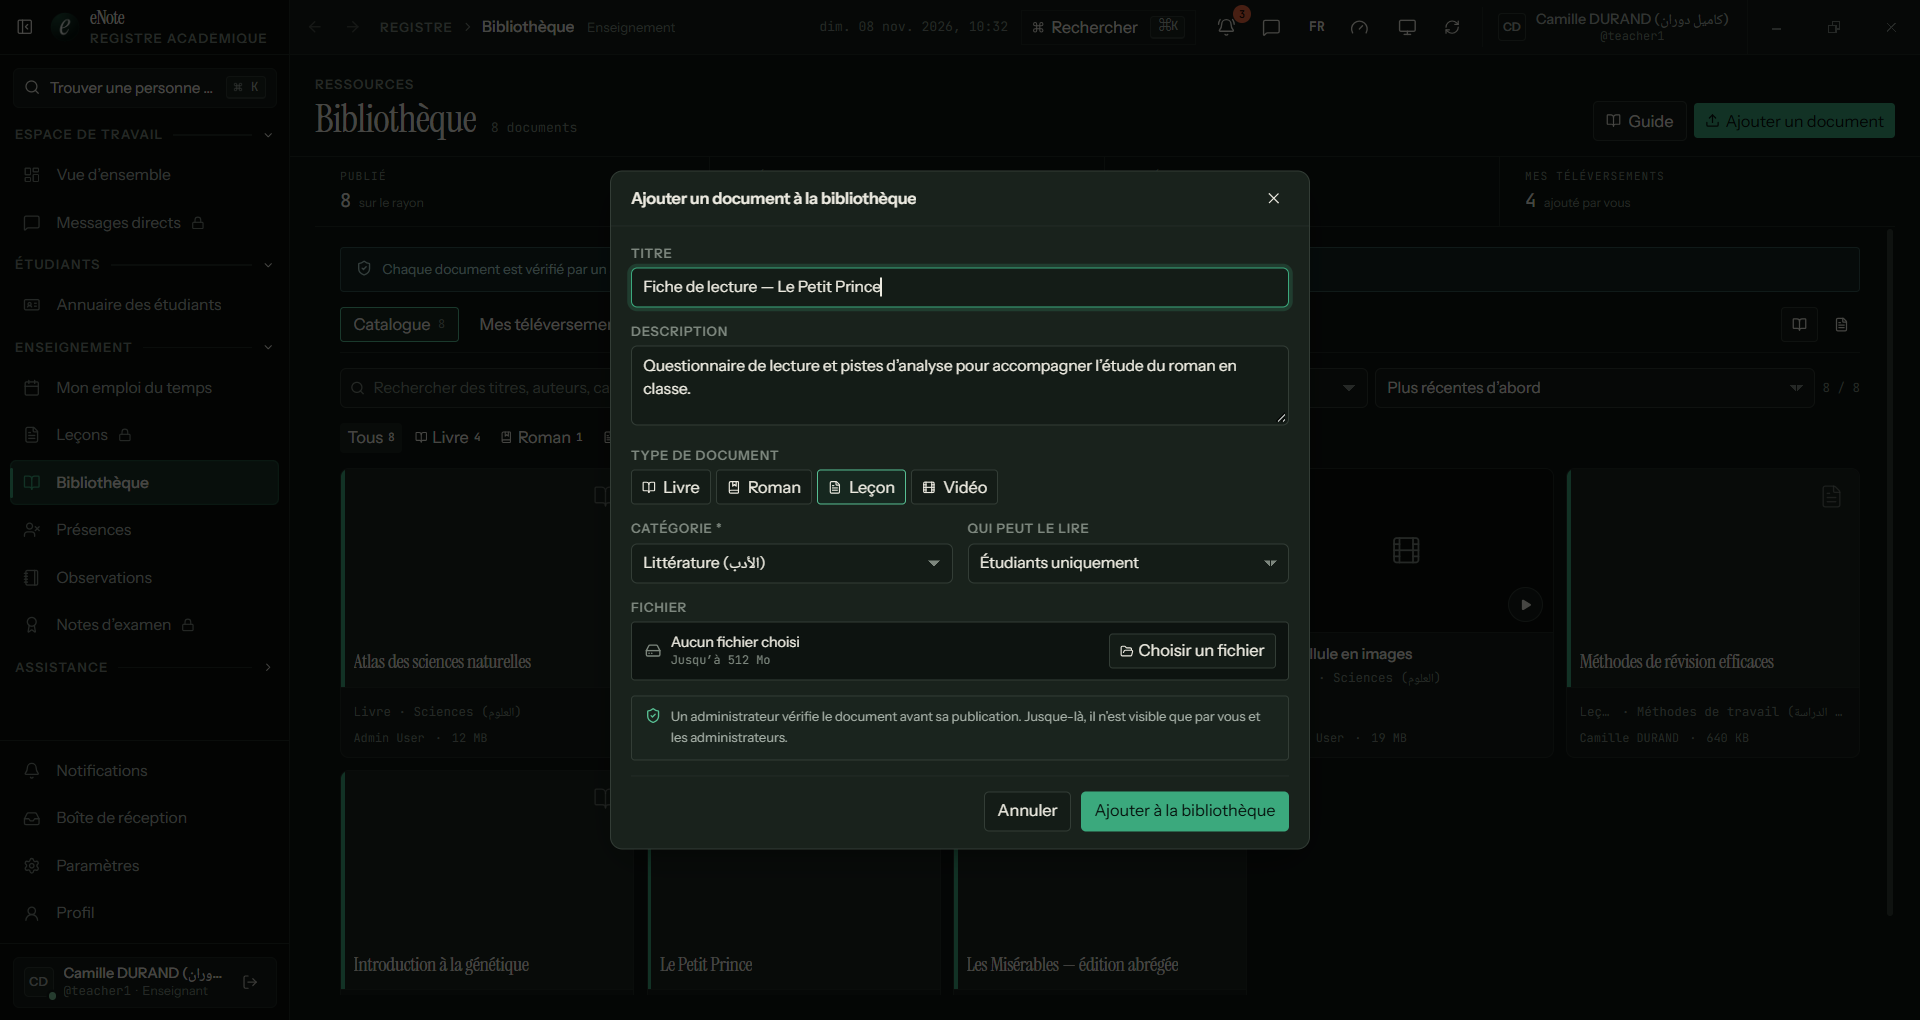
\includegraphics[width=0.85\textwidth]{images/enseignant_bibliotheque.png}}{\fbox{[[Capture : images/enseignant\_bibliotheque.png]]}}
    \caption{Dépôt d'un document dans la bibliothèque}
    \label{fig:enseignant_bibliotheque}
\end{figure}

\subsection{Consultation d'un dossier d'élève}
\textbf{Objectif :} connaître la situation d'un élève qu'on enseigne, sans modifier son dossier.\par
\textbf{Accès :} Menu > Élèves > \emph{Répertoire des élèves}.\par
\begin{enumerate}
    \item Rechercher l'élève par nom ou identifiant.
    \item Ouvrir le volet d'inspection pour lire les informations utiles.
    \item Consulter l'historique des absences et des observations depuis les pages de supervision
          autorisées.
\end{enumerate}
\textbf{Règles et contrôles :} l'enseignant lit le dossier mais ne peut ni l'inscrire, ni le corriger :
les actions d'écriture ne sont pas proposées, et le service les refuse. Le périmètre de lecture est
celui de l'établissement, pas celui de la classe, car un enseignant peut intervenir dans plusieurs
sections.\par
\textbf{Résultat attendu :} l'enseignant dispose du contexte nécessaire à son cours sans devenir un
administrateur de fait.

\begin{figure}[H]
    \centering
    \IfFileExists{images/enseignant_dossier.png}{\includegraphics[width=0.85\textwidth]{images/enseignant_dossier.png}}{\fbox{[[Capture : images/enseignant\_dossier.png]]}}
    \caption{Dossier d'un élève en lecture}
    \label{fig:enseignant_dossier}
\end{figure}

% ================================================================
% Bloc rôle : Étudiant
% ================================================================
\section{Guide d'Utilisation d'Étudiant}
\subsection{Consulter son emploi du temps}
\textbf{Objectif :} savoir où et quand se déroulent les cours de sa section.\par
\textbf{Accès :} Menu > Enseignement > \emph{Mon emploi du temps}.\par
\begin{enumerate}
    \item Choisir la semaine.
    \item Lire chaque cellule : type de séance, salle et enseignant.
    \item Changer de semaine si la grille est vide ; une explication est affichée sous la grille.
\end{enumerate}
\textbf{Règles et contrôles :} l'étudiant ne voit que les séances de ses sections ; une section non
affectée produit une grille vide expliquée, pas une erreur. Il ne peut pas modifier la grille.\par
\textbf{Résultat attendu :} l'étudiant connaît ses prochaines séances, sans démarche auprès du
secrétariat.

\begin{figure}[H]
    \centering
    \IfFileExists{images/etudiant_emploi.png}{\includegraphics[width=0.85\textwidth]{images/etudiant_emploi.png}}{\fbox{[[Capture : images/etudiant\_emploi.png]]}}
    \caption{Emploi du temps de l'étudiant}
    \label{fig:etudiant_emploi}
\end{figure}

\subsection{Consulter ses notes}
\textbf{Objectif :} lire ses notes, les moyennes par matière et sa moyenne semestrielle.\par
\textbf{Accès :} Menu > Enseignement > \emph{Mes notes}.\par
\begin{enumerate}
    \item Choisir l'année et le semestre.
    \item Lire les notes groupées par examen.
    \item Consulter la synthèse en haut de page : moyenne semestrielle et moyennes par matière.
\end{enumerate}
\textbf{Règles et contrôles :} l'étudiant ne voit que ses propres notes ; l'identifiant de la personne
vient de la session, pas d'un paramètre d'adresse. Une note non saisie apparaît en tiret et n'entre pas
dans la moyenne. La moyenne d'une filière pondère les examens par leur coefficient, et la moyenne
semestrielle pondère les filières par leur facteur semestriel.\par
\textbf{Résultat attendu :} l'étudiant voit ses résultats dès leur publication, avec une moyenne
explicable.

\begin{figure}[H]
    \centering
    \IfFileExists{images/etudiant_notes.png}{\includegraphics[width=0.85\textwidth]{images/etudiant_notes.png}}{\fbox{[[Capture : images/etudiant\_notes.png]]}}
    \caption{Notes et moyennes de l'étudiant}
    \label{fig:etudiant_notes}
\end{figure}

\subsection{Accéder aux supports de cours}
\textbf{Objectif :} retrouver les fichiers publiés par les enseignants.\par
\textbf{Accès :} Menu > Enseignement > \emph{Leçons}.\par
\begin{enumerate}
    \item Ouvrir une leçon depuis la liste.
    \item Lire la description et la liste des fichiers.
    \item Ouvrir, télécharger ou visionner un fichier ; les vidéos se lisent dans la page.
    \item Utiliser \emph{Enregistrer hors ligne} (icône disque) pour garder une copie du fichier sur
          l'ordinateur : elle s'ouvre pendant une panne du serveur ou du partage.
\end{enumerate}
\textbf{Règles et contrôles :} l'étudiant lit et visionne, mais n'ajoute ni ne retire de fichier. Le
cache hors ligne est limité à deux gigaoctets et s'élague du plus ancien, pour ne pas remplir le disque
d'un poste partagé. Un
fichier retiré par l'enseignant disparaît de la leçon ; un fichier déjà téléchargé reste sur le poste,
car l'application ne peut pas le reprendre.\par
\textbf{Résultat attendu :} l'étudiant dispose des supports à tout moment, sans accès Internet.

\begin{figure}[H]
    \centering
    \IfFileExists{images/etudiant_lecons.png}{\includegraphics[width=0.85\textwidth]{images/etudiant_lecons.png}}{\fbox{[[Capture : images/etudiant\_lecons.png]]}}
    \caption{Leçons et supports disponibles}
    \label{fig:etudiant_lecons}
\end{figure}

\subsection{Consulter la bibliothèque}
\textbf{Objectif :} lire les livres, romans, leçons et vidéos publiés pour les étudiants.\par
\textbf{Accès :} Menu > Enseignement > \emph{Bibliothèque}.\par
\begin{enumerate}
    \item Parcourir les rayons ou la liste, puis rechercher un titre ou une catégorie.
    \item Filtrer par type et ouvrir un document pour lire sa description et son auteur.
    \item Visionner une vidéo dans la page, ou ouvrir le document dans son application.
    \item Télécharger une copie si l'administration l'autorise.
    \item Enregistrer un document hors ligne pour le garder sur l'ordinateur et le lire pendant une
          panne ; la copie est datée et peut être oubliée depuis la même fiche.
\end{enumerate}
\textbf{Règles et contrôles :} l'étudiant ne voit que les documents publiés ouverts à tous ou aux
étudiants ; un dépôt en attente, rejeté ou réservé aux enseignants reste invisible. Il ne peut ni
ajouter, ni modifier, ni retirer un document. Le téléchargement peut être fermé par l'administration,
sans empêcher la lecture dans la page. Une vidéo est lue par le lecteur intégré, sans accès Internet.\par
\textbf{Résultat attendu :} l'étudiant dispose d'un catalogue de lecture stable, sans voir les documents
en cours de revue.

\begin{figure}[H]
    \centering
    \IfFileExists{images/etudiant_bibliotheque.png}{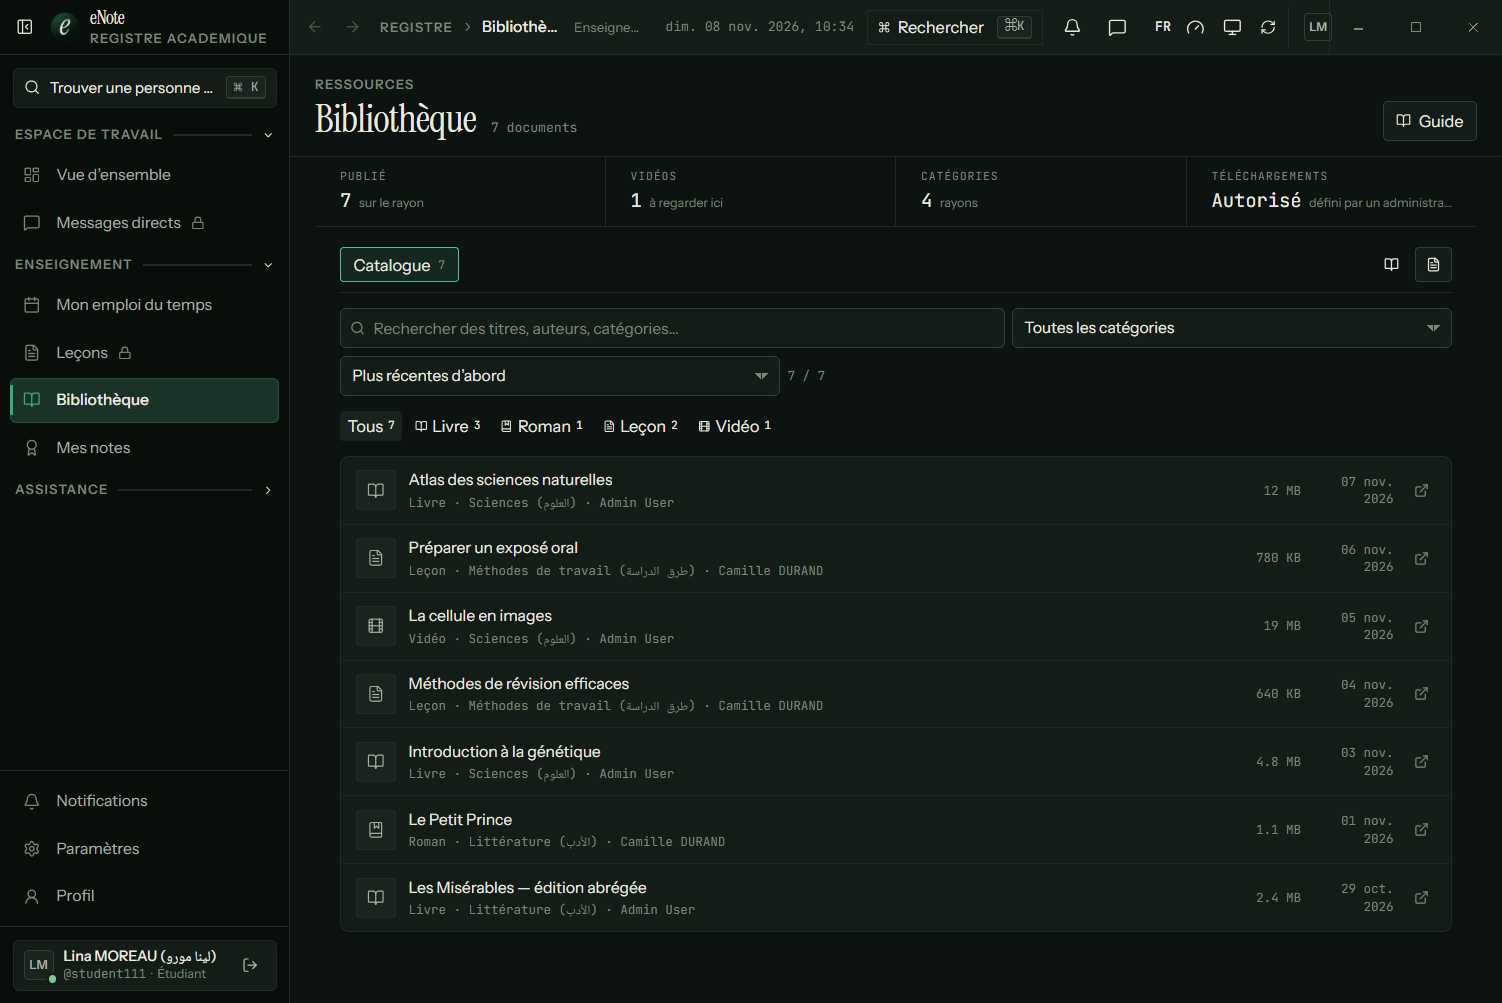
\includegraphics[width=0.85\textwidth]{images/etudiant_bibliotheque.png}}{\fbox{[[Capture : images/etudiant\_bibliotheque.png]]}}
    \caption{Bibliothèque vue par l'étudiant}
    \label{fig:etudiant_bibliotheque}
\end{figure}

\subsection{Notifications et messages}
\textbf{Objectif :} être informé d'un changement de salle, d'une note publiée ou d'un message.\par
\textbf{Accès :} pied de la barre latérale > \emph{Notifications} / \emph{Messages}.\par
\begin{enumerate}
    \item Ouvrir la cloche pour lire les notifications non lues.
    \item Suivre le lien d'une notification vers la page concernée.
    \item Utiliser \emph{Tout marquer comme lu} pour remettre le badge à zéro.
    \item Répondre dans la messagerie directe si la conversation le permet.
\end{enumerate}
\textbf{Règles et contrôles :} un étudiant ne reçoit pas les notifications de supervision réservées aux
adultes. La messagerie directe le met en relation avec les rôles autorisés par la matrice ; il ne peut
pas écrire à un rôle qui ne figure pas dans ses contacts. Les notifications système ne s'affichent que
si le poste les autorise.\par
\textbf{Résultat attendu :} l'étudiant est informé sans devoir consulter chaque page.

\begin{figure}[H]
    \centering
    \IfFileExists{images/etudiant_notifications.png}{\includegraphics[width=0.85\textwidth]{images/etudiant_notifications.png}}{\fbox{[[Capture : images/etudiant\_notifications.png]]}}
    \caption{Centre de notifications}
    \label{fig:etudiant_notifications}
\end{figure}

\subsection{Profil et photo}
\textbf{Objectif :} vérifier sa fiche et tenir sa photo à jour.\par
\textbf{Accès :} pied de la barre latérale > \emph{Profil}.\par
\begin{enumerate}
    \item Lire son nom, sa section et ses coordonnées.
    \item Changer la photo avec le sélecteur natif.
    \item Demander une correction d'état civil au secrétariat.
\end{enumerate}
\textbf{Règles et contrôles :} l'étudiant ne peut modifier que sa photo. Les informations d'identité
appartiennent au dossier tenu par le secrétariat, et une correction y laisse une trace. La photo
apparaît dans les listes de classe et dans les conversations.\par
\textbf{Résultat attendu :} la fiche de l'étudiant est à jour sans intervention du secrétariat pour la
photo.

\begin{figure}[H]
    \centering
    \IfFileExists{images/etudiant_profil.png}{\includegraphics[width=0.85\textwidth]{images/etudiant_profil.png}}{\fbox{[[Capture : images/etudiant\_profil.png]]}}
    \caption{Profil de l'étudiant}
    \label{fig:etudiant_profil}
\end{figure}

% ================================================================
% Bloc rôle : Planificateur
% ================================================================
\section{Guide d'Utilisation de Planificateur}
\subsection{Construction de l'emploi du temps}
\textbf{Objectif :} placer les séances d'une semaine dans les créneaux et les salles disponibles.\par
\textbf{Accès :} Menu > Supervision > \emph{Emploi du temps général}.\par
\begin{enumerate}
    \item Choisir l'année, le semestre et la semaine.
    \item Utiliser \emph{Créer une séance} et choisir le type, l'enseignant, la salle et le groupe.
    \item Lire les indications de conflit : un groupe, une salle ou un enseignant déjà occupé est
          signalé, et l'application propose le premier libre.
    \item Enregistrer ; la séance apparaît dans la grille et dans les emplois du temps individuels.
    \item Supprimer une séance depuis sa cellule pour la corriger.
\end{enumerate}
\textbf{Règles et contrôles :} un créneau déjà pris pour le groupe est refusé, et le jour choisi doit
appartenir à une semaine existante. Les conflits de salle et d'enseignant sont détectés sur le même
créneau, et les listes déroulantes les signalent avant l'enregistrement. Le planificateur ne peut agir
que dans les catégories d'enseignement qui lui sont attribuées ; une séance ou un groupe hors périmètre
est refusé par le service.\par
\textbf{Résultat attendu :} la grille est mise à jour et les emplois du temps des enseignants et des
étudiants suivent immédiatement.

\begin{figure}[H]
    \centering
    \IfFileExists{images/planificateur_emploi.png}{\includegraphics[width=0.85\textwidth]{images/planificateur_emploi.png}}{\fbox{[[Capture : images/planificateur\_emploi.png]]}}
    \caption{Emploi du temps général}
    \label{fig:planificateur_emploi}
\end{figure}

\subsection{Suivi des volumes horaires}
\textbf{Objectif :} comparer les heures programmées aux heures cibles d'un groupe.\par
\textbf{Accès :} Emploi du temps général > \emph{Volume}.\par
\begin{enumerate}
    \item Choisir le groupe et le semestre.
    \item Lire le volume cible par type de séance et par section.
    \item Comparer avec les heures déjà placées dans la grille.
    \item Ajuster la programmation ; un dépassement est refusé à l'enregistrement.
\end{enumerate}
\textbf{Règles et contrôles :} le contrôle du volume est effectué avant l'écriture : si la durée de la
séance dépasse les heures restantes pour ce type, l'application refuse et indique le nombre d'heures
déjà utilisées et le plafond. Le volume cible est défini par filière, semestre et type de séance, et
peut être affiné par section. Un volume à zéro signifie que le type n'est pas prévu, pas qu'il est
illimité.\par
\textbf{Résultat attendu :} un écart visible entre le programme prévu et les séances réellement
planifiées, avant que l'écart ne devienne un manque d'heures en fin de semestre.

\begin{figure}[H]
    \centering
    \IfFileExists{images/planificateur_volume.png}{\includegraphics[width=0.85\textwidth]{images/planificateur_volume.png}}{\fbox{[[Capture : images/planificateur\_volume.png]]}}
    \caption{Panneau des volumes horaires}
    \label{fig:planificateur_volume}
\end{figure}

\subsection{Programmation des examens}
\textbf{Objectif :} fixer la date, la filière, le coefficient et les surveillants d'un examen.\par
\textbf{Accès :} Menu > Enseignement > \emph{Examens}.\par
\begin{enumerate}
    \item Choisir l'année et le semestre, puis la filière.
    \item Utiliser \emph{Ajouter un examen} : code, libellés dans les trois langues, type, filière,
          semestre, début, fin et coefficient.
    \item Choisir les surveillants parmi le personnel libre pendant le créneau.
    \item Enregistrer, puis vérifier l'examen dans la liste filtrée.
\end{enumerate}
\textbf{Règles et contrôles :} la liste des surveillants est recalculée à chaque changement d'horaire :
une personne qui surveille ou passe un examen sur le même créneau n'est pas proposée. Un surveillant
est un membre du personnel, pas un étudiant. Les filtres de la liste portent sur le semestre, le type,
la période (à venir, passée), l'état de la disposition et la présence du coefficient.\par
\textbf{Résultat attendu :} l'examen est programmé avec des surveillants disponibles, et la liste
signale les données manquantes avant la date.

\begin{figure}[H]
    \centering
    \IfFileExists{images/planificateur_examens.png}{\includegraphics[width=0.85\textwidth]{images/planificateur_examens.png}}{\fbox{[[Capture : images/planificateur\_examens.png]]}}
    \caption{Programmation d'un examen}
    \label{fig:planificateur_examens}
\end{figure}

\subsection{Disposition en salle}
\textbf{Objectif :} répartir les candidats en groupes, leur attribuer une place et un code de copie.\par
\textbf{Accès :} liste des examens > \emph{Gérer la disposition}.\par
\begin{enumerate}
    \item Choisir la taille des groupes, puis mélanger les étudiants.
    \item Attribuer une salle à chaque groupe.
    \item Attribuer une place à chaque étudiant dans la salle du groupe.
    \item Renseigner le code de copie de chaque candidat.
    \item Enregistrer la disposition.
\end{enumerate}
\textbf{Règles et contrôles :} une place doit exister dans la salle choisie ; une place ne peut pas être
attribuée à deux étudiants de la même salle. Un code de copie doit être unique dans l'examen et ne peut
pas être réutilisé dans un autre examen. La composition des groupes est enregistrée, ce qui permet de
retrouver la salle et la place d'un candidat le jour de l'épreuve. Les étudiants sans section ou sans
groupe ne peuvent pas être placés et sont signalés.\par
\textbf{Résultat attendu :} chaque candidat connaît sa salle, sa place et son code, et aucun conflit de
place ou de code ne subsiste.

\begin{figure}[H]
    \centering
    \IfFileExists{images/planificateur_places.png}{\includegraphics[width=0.85\textwidth]{images/planificateur_places.png}}{\fbox{[[Capture : images/planificateur\_places.png]]}}
    \caption{Disposition des candidats en salle}
    \label{fig:planificateur_places}
\end{figure}

\subsection{Consultation des notes et des moyennes}
\textbf{Objectif :} contrôler les résultats d'un examen et les moyennes semestrielles d'une filière.\par
\textbf{Accès :} Menu > Enseignement > \emph{Notes d'examen}.\par
\begin{enumerate}
    \item Basculer entre \emph{Notes} et \emph{Moyennes semestrielles}.
    \item Choisir l'examen ou la filière à examiner.
    \item Vérifier les notes manquantes et les coefficients appliqués.
    \item Signaler à l'enseignant concerné toute anomalie ; la saisie reste son travail.
\end{enumerate}
\textbf{Règles et contrôles :} le planificateur consulte mais ne saisit pas les notes ; la saisie est
réservée à l'enseignant de la filière. Une note vide est exclue de la moyenne, et le coefficient de
l'examen comme le facteur de la filière sont rappelés à l'écran pour rendre le calcul vérifiable.\par
\textbf{Résultat attendu :} une vue consolidée des résultats, cohérente avec les coefficients définis
pour la filière et le semestre.

\begin{figure}[H]
    \centering
    \IfFileExists{images/planificateur_notes.png}{\includegraphics[width=0.85\textwidth]{images/planificateur_notes.png}}{\fbox{[[Capture : images/planificateur\_notes.png]]}}
    \caption{Moyennes semestrielles d'une filière}
    \label{fig:planificateur_notes}
\end{figure}

% ================================================================
% Bloc rôle : Développeur
% ================================================================
\section{Guide d'Utilisation de Développeur}
\subsection{Traitement des rapports d'anomalie}
\textbf{Objectif :} trier les problèmes signalés par les utilisateurs et suivre leur résolution.\par
\textbf{Accès :} Menu > Support > \emph{Rapports d'anomalie}.\par
\begin{enumerate}
    \item Lire la file, du plus récent au plus ancien, ou filtrer par statut.
    \item Rechercher un rapport par mot-clé.
    \item Ouvrir un rapport et changer son statut : \emph{Ouvert}, \emph{En cours}, \emph{Résolu},
          \emph{Rejeté}.
    \item Changer la priorité : \emph{Basse}, \emph{Moyenne}, \emph{Élevée}, \emph{Critique}.
    \item Utiliser \emph{Rafraîchir} pour récupérer les nouveaux signalements sans quitter la page.
\end{enumerate}
\textbf{Règles et contrôles :} le statut et la priorité sont stockés en anglais et affichés dans la
langue de l'interface. Chaque changement est enregistré contre le compte qui l'a effectué. La capture
d'écran jointe est ouverte par le processus principal, jamais par un lien fourni par la page. La liste
est paginée, et la recherche combine le texte libre et le filtre de statut.\par
\textbf{Résultat attendu :} chaque rapport a un statut à jour et l'auteur retrouve l'avancement dans
\emph{Mes rapports}.

\begin{figure}[H]
    \centering
    \IfFileExists{images/developpeur_anomalies.png}{\includegraphics[width=0.85\textwidth]{images/developpeur_anomalies.png}}{\fbox{[[Capture : images/developpeur\_anomalies.png]]}}
    \caption{File de traitement des anomalies}
    \label{fig:developpeur_anomalies}
\end{figure}

\subsection{Exploitation des rapports de test bêta}
\textbf{Objectif :} décider ce qui sera corrigé avant la publication d'une version.\par
\textbf{Accès :} Menu > Support > \emph{Rapports de test bêta}.\par
\begin{enumerate}
    \item Choisir une version.
    \item Filtrer : tous les rapports, ceux qui contiennent des problèmes, ou ceux où toutes les
          fonctionnalités ont été testées.
    \item Lire, pour chaque testeur, le nombre de fonctionnalités testées, le nombre de problèmes et la
          gravité la plus élevée.
    \item Lire le commentaire général et les descriptions de problèmes.
\end{enumerate}
\textbf{Règles et contrôles :} un rapport est unique par testeur et par version. La gravité la plus
élevée d'un rapport est calculée à partir des problèmes déclarés (critique, élevée, moyenne, basse), ce
qui permet de trier les versions à risque. Un testeur qui n'a rien signalé reste visible : l'absence de
problème est une information.\par
\textbf{Résultat attendu :} une décision de publication appuyée sur des retours datés et nominatifs.

\begin{figure}[H]
    \centering
    \IfFileExists{images/developpeur_beta.png}{\includegraphics[width=0.85\textwidth]{images/developpeur_beta.png}}{\fbox{[[Capture : images/developpeur\_beta.png]]}}
    \caption{Synthèse des tests bêta}
    \label{fig:developpeur_beta}
\end{figure}

\subsection{Rédaction des notes de version}
\textbf{Objectif :} informer les utilisateurs de ce qui change à chaque publication.\par
\textbf{Accès :} Menu > Support > \emph{Journal des modifications}.\par
\begin{enumerate}
    \item Utiliser \emph{Nouvelle version} et renseigner le numéro, la date et les notes.
    \item Saisir les notes dans les trois langues : l'anglais sert de repli aux deux autres.
    \item Enregistrer, puis relire l'entrée telle qu'elle apparaîtra aux utilisateurs.
    \item Ouvrir une entrée pour la corriger ou la supprimer.
\end{enumerate}
\textbf{Règles et contrôles :} une version publiée est présentée une fois à chaque compte, dans une
fenêtre dédiée ; l'acquittement est propre au compte, pas au poste. Les notes sont du contenu libre :
elles ne sont pas traduites automatiquement, et une note laissée vide dans une langue s'affiche en
anglais. La suppression d'une entrée ne supprime pas les rapports de test qui la référencent.\par
\textbf{Résultat attendu :} une note de version datée, traduite, visible par tous les comptes.

\begin{figure}[H]
    \centering
    \IfFileExists{images/developpeur_changelog.png}{\includegraphics[width=0.85\textwidth]{images/developpeur_changelog.png}}{\fbox{[[Capture : images/developpeur\_changelog.png]]}}
    \caption{Édition d'une note de version}
    \label{fig:developpeur_changelog}
\end{figure}

\subsection{Journal d'activité}
\textbf{Objectif :} comprendre une anomalie en retrouvant l'action et l'acteur qui l'ont précédée.\par
\textbf{Accès :} Menu > Support > \emph{Journal d'activité}.\par
\begin{enumerate}
    \item Filtrer par période, acteur, action, type d'entité ou résultat.
    \item Rechercher un nom, une action ou un message d'erreur.
    \item Ouvrir le détail d'une entrée pour lire les valeurs avant et après.
    \item Exporter le sous-ensemble filtré au format \ac{CSV}.
\end{enumerate}
\textbf{Règles et contrôles :} le journal est en ajout seul et ne peut être modifié depuis
l'application ; les entrées de plus de douze mois sont élaguées. Les échecs de connexion y figurent avec
leur motif, mais jamais le mot de passe essayé. L'export est plafonné et porte sur les filtres actifs.\par
\textbf{Résultat attendu :} un diagnostic reproductible et une trace exploitable, sans altération
possible.

\begin{figure}[H]
    \centering
    \IfFileExists{images/developpeur_journal.png}{\includegraphics[width=0.85\textwidth]{images/developpeur_journal.png}}{\fbox{[[Capture : images/developpeur\_journal.png]]}}
    \caption{Journal d'activité et détail d'une entrée}
    \label{fig:developpeur_journal}
\end{figure}

\subsection{Console de diagnostic de la base}
\textbf{Objectif :} vérifier la connexion et contrôler une valeur sans passer par un outil externe.\par
\textbf{Accès :} Menu > Support > \emph{Base de données}.\par
\begin{enumerate}
    \item Lire l'état de la connexion, l'hôte, le port et la base utilisés.
    \item Choisir une table pour parcourir ses colonnes et ses lignes.
    \item Exécuter une requête de lecture dans la console.
    \item Quitter la page pour revenir à l'application.
\end{enumerate}
\textbf{Règles et contrôles :} la console est en lecture seule ; aucune écriture n'est proposée, même à
un développeur. Le mot de passe de connexion n'est jamais affiché. La page est réservée aux rôles
administrateur et développeur, et chaque accès est tracé.\par
\textbf{Résultat attendu :} un diagnostic reproductible, sans donner à l'application un rôle d'éditeur
de base.

\begin{figure}[H]
    \centering
    \IfFileExists{images/developpeur_diagnostic.png}{\includegraphics[width=0.85\textwidth]{images/developpeur_diagnostic.png}}{\fbox{[[Capture : images/developpeur\_diagnostic.png]]}}
    \caption{Console de diagnostic de la base}
    \label{fig:developpeur_diagnostic}
\end{figure}

\subsection{Comptes et paramètres techniques}
\textbf{Objectif :} intervenir sur les comptes et les options techniques sans disposer des droits
d'administration complets.\par
\textbf{Accès :} Menu > Comptes et accès > \emph{Comptes}, et \emph{Paramètres > Administration}.\par
\begin{enumerate}
    \item Rechercher un compte, l'activer ou le désactiver, et changer son nom d'utilisateur, son
          courriel, son mot de passe ou son rôle.
    \item Consulter les pages verrouillées et les permissions de message.
    \item Accéder au registre hérité pour une reprise de données, après prévisualisation.
\end{enumerate}
\textbf{Règles et contrôles :} le rôle développeur gère les comptes, mais pas le registre des personnes,
les comptes secrétaires ni les suspensions, qui restent des tâches d'administration. Il ne peut pas
changer l'état ni le rôle de son propre compte, et ne peut pas retirer le rôle Admin au dernier
administrateur actif. Les options globales applicatives restent réservées à l'administrateur.\par
\textbf{Résultat attendu :} les interventions techniques sont possibles sans élargir le rôle développeur
à toute l'administration.

\begin{figure}[H]
    \centering
    \IfFileExists{images/developpeur_comptes.png}{\includegraphics[width=0.85\textwidth]{images/developpeur_comptes.png}}{\fbox{[[Capture : images/developpeur\_comptes.png]]}}
    \caption{Comptes et options techniques}
    \label{fig:developpeur_comptes}
\end{figure}

\section{Conclusion}
Ce chapitre a présenté l'installation du serveur et des postes, les fonctionnalités transverses puis
les gestes propres à chaque rôle, avec pour chaque écran son objectif, son accès, ses prérequis, ses
étapes, ses règles de refus et son résultat attendu. Le lecteur dispose ainsi d'un mode d'emploi
complet : un technicien peut déployer l'application sur un réseau isolé, un administrateur peut ouvrir
une année scolaire, et chaque utilisateur trouve la procédure qui correspond à sa responsabilité, du
premier appel de la journée à la génération d'un rapport officiel, et de la consultation d'un support
à la revue d'un document de la bibliothèque.
